% arxiv-twocolumn.latex: the shared pandoc template for a two-column arXiv-style preprint.
% Built by build_paper.py (pandoc, then tectonic or any XeLaTeX); arxiv-twocolumn.lua is its filter.
% Engine: XeTeX (fontspec, unicode-math). Fonts: Latin Modern text and math, DejaVu Sans Mono for code;
% a character the current font lacks falls back to Latin Modern Math, then to DejaVu Sans.
\documentclass[10pt,letterpaper,twocolumn]{article}
\usepackage[letterpaper,top=0.75in,bottom=0.9in,left=0.7in,right=0.7in,columnsep=0.25in]{geometry}
\usepackage{amsmath}
\usepackage{fontspec}
\usepackage{unicode-math}
\setmainfont{lmroman10}[Extension=.otf,UprightFont=*-regular,BoldFont=*-bold,ItalicFont=*-italic,BoldItalicFont=*-bolditalic]
\setsansfont{lmsans10}[Extension=.otf,UprightFont=*-regular,BoldFont=*-bold,ItalicFont=*-oblique,BoldItalicFont=*-boldoblique]
\setmonofont{DejaVuSansMono}[Extension=.ttf,UprightFont=*,BoldFont=*-Bold,ItalicFont=*-Oblique,BoldItalicFont=*-BoldOblique,Scale=MatchLowercase]
\setmathfont{latinmodern-math.otf}
\newfontfamily\typesetfallbackmath{latinmodern-math.otf}
\newfontfamily\typesetfallbacksans{DejaVuSans}[Extension=.ttf,UprightFont=*,BoldFont=*-Bold,ItalicFont=*-Oblique,BoldItalicFont=*-BoldOblique]
% \typesetmap{"XXXX} (build_paper.py writes one for each character outside Latin-1 and Latin
% Extended-A that the paper uses) makes the character active at the start of the document: in text it
% comes from the current font when that has it, else from the first fallback that does; in math it
% keeps whatever unicode-math gave it (a prime stays a prime).
\makeatletter
\protected\def\typesetglyph#1{%
  \iffontchar\font#1\relax\char#1\relax
  \else{\typesetfallbackmath\iffontchar\font#1\relax\char#1\relax\else\typesetfallbacksans\char#1\relax\fi}%
  \fi}
\def\typeset@math#1{%
  \ifcsname typeset@m@#1\endcsname\csname typeset@m@#1\expandafter\endcsname\else\Uchar#1 \fi}
\protected\def\typesetchar#1{\ifmmode\expandafter\typeset@math\else\expandafter\typesetglyph\fi{#1}}
\def\typesetmap#1{%
  \edef\typeset@n{\number#1}% outside \lowercase, which would lowercase the hex digits A-F
  \begingroup\lccode`\~=\typeset@n\relax
  \lowercase{\endgroup
    \ifdefined~\expandafter\let\csname typeset@m@\typeset@n\endcsname~\fi
    \edef~{\noexpand\typesetchar{\typeset@n}}}%
  \catcode\typeset@n=13\relax}
\makeatother
% amssymb names that unicode-math spells differently.
\AtBeginDocument{%
  \providecommand{\square}{\mdlgwhtsquare}\providecommand{\Box}{\mdlgwhtsquare}%
  \providecommand{\blacksquare}{\mdlgblksquare}\providecommand{\lozenge}{\mdlgwhtlozenge}%
  \providecommand{\blacklozenge}{\mdlgblklozenge}}
% Legacy two-letter font commands (\rm, \bf, \it, ...), in text and in math.
\providecommand{\rm}{}\DeclareOldFontCommand{\rm}{\normalfont\rmfamily}{\mathrm}
\providecommand{\bf}{}\DeclareOldFontCommand{\bf}{\normalfont\bfseries}{\mathbf}
\providecommand{\it}{}\DeclareOldFontCommand{\it}{\normalfont\itshape}{\mathit}
\providecommand{\sf}{}\DeclareOldFontCommand{\sf}{\normalfont\sffamily}{\mathsf}
\providecommand{\tt}{}\DeclareOldFontCommand{\tt}{\normalfont\ttfamily}{\mathtt}
\usepackage{microtype}
\usepackage[dvipsnames]{xcolor}
\usepackage{graphicx}
\usepackage{booktabs}
\usepackage{array}
\usepackage{ragged2e}
\usepackage{xtab}
\usepackage{cuted}
\usepackage{caption}
\captionsetup{font=small,labelfont=bf,skip=4pt}
\captionsetup[table]{position=top}
\usepackage{fvextra}
\usepackage{xurl}
\usepackage{titlesec}
\usepackage{fancyhdr}
\usepackage{footmisc}
\usepackage{enumitem}
\setlist{itemsep=1pt,topsep=3pt,parsep=0pt}
\usepackage{hyperref}
\hypersetup{colorlinks=true,linkcolor=MidnightBlue,citecolor=MidnightBlue,urlcolor=MidnightBlue,filecolor=MidnightBlue,
  pdftitle={Entroptics},pdfauthor={Ikailo John Sessford},pdfcreator={pandoc + XeTeX},bookmarksnumbered=true}
\pdfstringdefDisableCommands{\def\typesetchar#1{\Uchar#1 }}

% Paragraphs: indented, no extra space, ragged bottom so columns do not stretch.
\setlength{\parskip}{0pt}
\raggedbottom
\emergencystretch=1.5em
\tolerance=1000
\hbadness=10000
\clubpenalty=10000
\widowpenalty=10000

% Section headings. Numbered only when the paper's own headings carry no numbers (build_paper.py decides).
\setcounter{secnumdepth}{-\maxdimen}
\titleformat*{\section}{\normalfont\large\bfseries\raggedright}
\titleformat*{\subsection}{\normalfont\normalsize\bfseries\raggedright}
\titleformat*{\subsubsection}{\normalfont\normalsize\bfseries\itshape\raggedright}
\titleformat*{\paragraph}{\normalfont\normalsize\itshape}
\titlespacing*{\section}{0pt}{2.0ex plus 1ex minus .2ex}{1.0ex plus .2ex}
\titlespacing*{\subsection}{0pt}{1.6ex plus 1ex minus .2ex}{0.6ex plus .2ex}
\titlespacing*{\subsubsection}{0pt}{1.4ex plus 1ex minus .2ex}{0.5ex plus .2ex}
\titlespacing*{\paragraph}{0pt}{1.0ex plus .5ex}{0.6em}

% Code: monospaced at the floor size, wrapped at the column edge and never scaled.
\RecustomVerbatimEnvironment{verbatim}{Verbatim}{fontsize=\footnotesize,breaklines=true,breakanywhere=true,breaksymbolleft={},
  xleftmargin=0.5em,frame=leftline,framerule=0.4pt,rulecolor=\color{Gray},framesep=0.5em}

% Tables: small type, tight columns. Long tables break across columns (xtabular); wide ones float full width.
\setlength{\tabcolsep}{4pt}
\renewcommand{\arraystretch}{1.1}
\newcolumntype{L}[1]{>{\RaggedRight\arraybackslash}p{#1}}
\newcolumntype{R}[1]{>{\RaggedLeft\arraybackslash}p{#1}}
\newcolumntype{C}[1]{>{\Centering\arraybackslash}p{#1}}
% Scaling has a floor: nothing is set smaller than \typesetfloor.
% DERIVED: 8 pt is \footnotesize of this 10 pt class, the smallest running text the template sets
% (tables, code), so a scaled display is never smaller than the smallest text already on the page.
\newdimen\typesetfloor \typesetfloor=8pt
\newsavebox{\typesetfitbox}
\newif\iftypesetfitok
\makeatletter
% \typeset@try{width}{base size}: does \typesetfitbox fit in width, scaled no smaller than the floor?
% Sets \iftypesetfitok, and logs the scale it would apply ("typeset-scale: <scale x 1000>").
\def\typeset@try#1#2{%
  \ifdim\wd\typesetfitbox>#1\relax
    \edef\typeset@scale{\the\numexpr\number\dimexpr#1\relax*1000/\number\wd\typesetfitbox\relax}%
    % the effective size, base size x scale, against the floor
    \ifdim\dimexpr#2*\typeset@scale/1000\relax<\typesetfloor
      \typesetfitokfalse
    \else
      \typesetfitoktrue\typeout{typeset-scale: \typeset@scale}%
    \fi
  \else
    \typesetfitoktrue
  \fi}
% \typesetfit{width}{content}: the content at natural size, scaled down only when wider than width,
% and never below the floor; content too wide even at the floor is set at the floor and overflows,
% which the build reports ("typeset-overflow").
\newcommand{\typesetfit}[2]{\sbox{\typesetfitbox}{#2}\typeset@place{#1}{\f@size pt}}
\def\typeset@place#1#2{%
  \typeset@try{#1}{#2}%
  \iftypesetfitok
    \ifdim\wd\typesetfitbox>#1\relax\resizebox{#1}{!}{\usebox{\typesetfitbox}}\else\usebox{\typesetfitbox}\fi
  \else
    \edef\typeset@floorscale{\the\numexpr\number\typesetfloor*1000/\number\dimexpr#2\relax\relax}%
    \ifnum\typeset@floorscale<1000
      \typeout{typeset-scale: \typeset@floorscale}%
      \scalebox{\strip@pt\dimexpr\typeset@floorscale pt/1000\relax}{\usebox{\typesetfitbox}}%
    \else
      \usebox{\typesetfitbox}%
    \fi
    \typeout{typeset-overflow: \the\wd\typesetfitbox\space into \the\dimexpr#1\relax}%
  \fi}
% \typesetdisplay{math}{split}: a display equation, and the same equation broken into lines at its
% top-level \qquad separators (empty when it has none). The first of these that fits, never below the
% floor, is used: the equation in the column; the split form in the column; the equation across both
% columns (a strip at this point of the text); the split form across both columns.
\def\typeset@show{%
  \[\ifdim\wd\typesetfitbox>\linewidth\resizebox{\linewidth}{!}{\usebox{\typesetfitbox}}\else\usebox{\typesetfitbox}\fi\]}
\def\typeset@strip{%
  \typeout{typeset-strip: display}%
  \par\begin{strip}\vspace{-\abovedisplayskip}\[\typeset@place{\textwidth}{\f@size pt}\]\vspace{-\belowdisplayskip}\end{strip}%
  \noindent\ignorespaces}
\long\def\typesetdisplay#1#2{%
  \sbox{\typesetfitbox}{\(\displaystyle #1\)}%
  \typeset@try{\linewidth}{\f@size pt}%
  \iftypesetfitok\typeset@show\else
    \long\def\typeset@alt{#2}%
    \ifx\typeset@alt\@empty\typeset@strip\else
      \sbox{\typesetfitbox}{\(\displaystyle #2\)}%
      \typeset@try{\linewidth}{\f@size pt}%
      \iftypesetfitok\typeset@show\else
        \sbox{\typesetfitbox}{\(\displaystyle #1\)}%
        \typeset@try{\textwidth}{\f@size pt}%
        \iftypesetfitok\else\sbox{\typesetfitbox}{\(\displaystyle #2\)}\fi
        \typeset@strip
      \fi
    \fi
  \fi}
% \typesetcolumntable{tabular}: an in-column table at natural size, in the column if it fits there
% (tables are already at the floor size, so they are never scaled), otherwise across both columns.
\long\def\typesetcolumntable#1{%
  \sbox{\typesetfitbox}{\footnotesize #1}%
  \ifdim\wd\typesetfitbox>\linewidth
    \typeout{typeset-strip: table}%
    \begin{strip}\centering\typeset@place{\textwidth}{\typesetfloor}\par\end{strip}%
  \else
    \begin{center}\usebox{\typesetfitbox}\end{center}%
  \fi}
\makeatother

% For the build's report: how full each column is when it is made ("typeset-column: page columns
% text floats height", lengths in sp). Float-only pages are made elsewhere and are not logged.
\usepackage{etoolbox}
\makeatletter
\def\typeset@colfill{%
  \setbox\z@\vbox{\unvcopy\@cclv}%
  \typeout{typeset-column: \number\c@page\space\if@twocolumn 2\else 1\fi\space
    \number\dimexpr\ht\z@+\dp\z@+\ht\footins+\dp\footins\relax\space
    \number\dimexpr\textheight-\@colroom\relax\space\number\textheight}}
\pretocmd{\@makecol}{\typeset@colfill}{}{\typeout{typeset-column: unavailable}}
% A heading above the paper's section level (a part of the paper) is set as a centred divider.
\newcounter{typesetpart}
\newcommand{\typesetpart}[2]{\par\vspace{2.5ex plus 1ex}\stepcounter{typesetpart}%
  \pdfbookmark[0]{#2}{typesetpart.\arabic{typesetpart}}%
  {\centering\large\bfseries #1\par}\vspace{1.5ex plus .5ex}}
\makeatother

% Floats: allow full-width floats to take most of a page, and many to queue.
\renewcommand{\topfraction}{0.9}
\renewcommand{\bottomfraction}{0.8}
\renewcommand{\textfraction}{0.07}
\renewcommand{\floatpagefraction}{0.75}
\renewcommand{\dbltopfraction}{0.9}
\renewcommand{\dblfloatpagefraction}{0.75}
\setcounter{topnumber}{3}
\setcounter{dbltopnumber}{3}
\setcounter{totalnumber}{5}
\extrafloats{200}
\setkeys{Gin}{width=\linewidth,height=0.8\textheight,keepaspectratio}

% Pandoc helpers.
\providecommand{\tightlist}{\setlength{\itemsep}{0pt}\setlength{\parskip}{0pt}}
\providecommand{\pandocbounded}[1]{#1}
\newcommand{\passthrough}[1]{#1}

\pagestyle{fancy}
\fancyhf{}
\renewcommand{\headrulewidth}{0pt}
\fancyfoot[C]{\small\thepage}
\fancypagestyle{plain}{\fancyhf{}\renewcommand{\headrulewidth}{0pt}\fancyfoot[C]{\small\thepage}}

\AtBeginDocument{%
\typesetmap{"220E}% ∎
\typesetmap{"22A2}% ⊢
}

\begin{document}

% Title block across both columns, with the abstract under it when the two leave room for the body to
% start on page 1; otherwise the abstract opens the two-column body, so no page is left near-empty.
\makeatletter
\newsavebox{\typesettitle}
\newsavebox{\typesetfront}
\setbox\typesettitle=\vbox{%
  \hsize=\textwidth \linewidth=\textwidth \columnwidth=\textwidth
  \begingroup\centering
  {\LARGE\bfseries Entroptics\par}
  \vspace{0.8ex}{\large Reading a 2-D signal as a finite optical aperture at its own entropy-matched resolution.\par}
  \vspace{1.8ex}
  {\normalsize Ikailo John Sessford\par}
  \vspace{0.3ex}
  {\small\itshape Ikailo Inc.\par}
  {\small \href{mailto:john@ikailo.com}{\texttt{john@ikailo.com}}\quad ORCID \href{https://orcid.org/0009-0002-0150-4027}{0009-0002-0150-4027}\par}
  \vspace{0.6ex}{\small Pre-print. November 2026.\par}
  \endgroup
}
\long\def\typesetrule{\vspace{1.6ex}\noindent\rule{\linewidth}{0.4pt}\par\vspace{1.5ex}}
\long\def\typesetabstract{%
We treat a two-dimensional signal \(W\in\mathbb{C}^{T\times F}\), with one \textbf{ordered} axis and one \textbf{feature} axis whose channels are commensurate, as a finite optical aperture whose resolution the signal's own Shannon entropy sets. From the entropy of the power marginals we read a matched scale; from the singular and correlation spectra, the standard optical quantities (fill fraction, étendue, Strehl ratio, space--bandwidth product); from the signal's own autocorrelation (a direct lag average, via Wiener--Khinchin), the optical transfer function (OTF) and, through the Abbe/Rayleigh relation, a diffraction limit. A streaming online dynamic mode decomposition (DMD) operator supplies the per-mode decay rates that the entropy width approximates, and a read-side filter --- the orthogonal projection onto the resolved modes above the derived floor, with a geometric persistent-structure cut --- splits the field losslessly into its own resolved modes and a residual, introducing no direction the data does not carry. Every read is defined from \(W\) alone and the construction is \textbf{parameter-free}: no constant anywhere is fitted to data or calibrated to a substrate, each being a derived mathematical quantity or a stated criterion, tabulated in §11.1. What the reader supplies is an operating point rather than a tuning --- a decision-risk level \(\alpha\), which by Neyman--Pearson encodes the cost of a false alarm against a miss and cannot be derived from the data, and the null it is taken against. Three further quantities are declared where a single record does not supply them: the forgetting factor \(\lambda\), stationary at \(\lambda=1\); the delay depth \(d\) of the Takens lift; and the signal-rank cut in the under-determined regime, taken at the §8 floor. Two declarations concern the record itself: which axis is ordered, and that the feature channels are commensurate. The distributional assumptions are the i.i.d. Gaussian bulk null of the noise-floor read (§§6, 8), row exchangeability for the permutation nulls (§5), channel independence for the estimator spread of Definition 4.8, and wide-sense stationarity for the Mercer ratio (§4.3) and the rates (§9). The provenance of every constant is tabulated in §11.1. We give precise definitions and prove the governing lemmas --- positive semidefiniteness of the biased autocovariance (hence a peak-at-zero-lag OTF), the fill-fraction and Strehl bounds, the scale-invariance of the Rayleigh shape factor, the permutation-null mean of the coherence statistic, a Weyl-certified interval for the attenuation constant, the recovery of the decay rates and the additivity behind stream splicing, and the axial/directional dichotomy of the concentration reads --- and tie each read to a named theorem in a term-by-term dictionary. The construction is realised in a small, backend-agnostic (numpy or torch), deterministic Python library whose test suite pins these identities, and is accompanied by a Lean 4 / Mathlib certification of the governing lemmas.
}
\setbox\typesetfront=\vbox{%
  \hsize=\textwidth \linewidth=\textwidth \columnwidth=\textwidth
  \unvcopy\typesettitle
  \vspace{2ex}
  {\centering\small\bfseries Abstract\par}
  \vspace{0.6ex}
  \begin{list}{}{\setlength{\leftmargin}{0.06\textwidth}\setlength{\rightmargin}{0.06\textwidth}%
    \setlength{\listparindent}{1.2em}\setlength{\itemindent}{0pt}\setlength{\parsep}{0.5ex}\setlength{\topsep}{0pt}}
  \small\item\relax\typesetabstract
  \end{list}
  \typesetrule
}
% CHOSEN: the title block and abstract go across both columns only if they leave ten lines of each
% column for the body on page 1. Ten lines is about a sixth of the page: enough that page 1 reads as
% the start of the paper, small enough that only a long abstract moves into the columns.
\ifdim\dimexpr\ht\typesetfront+\dp\typesetfront+10\baselineskip\relax<\textheight
  \twocolumn[\unvbox\typesetfront]
\else
  \twocolumn[\unvbox\typesettitle\typesetrule]
  {\centering\small\bfseries Abstract\par}\vspace{0.6ex}
  {\small\setlength{\parskip}{0.5ex}\noindent\typesetabstract\par}
  \typesetrule
\fi
\makeatother

\section{1. Introduction}\label{1-introduction}

Describing a field through the language of optics is an old experimental practice: free-space microwave measurements characterise a physical \emph{screen} by its reflection, attenuation, and diffraction, read at varying angles and distances, in optical terms {[}Kassner 1950{]}. The optical picture we take literally for data is the finite aperture: classically, it cannot resolve to infinitely fine detail --- its size fixes a diffraction limit, and the image is the object convolved with the aperture's point-spread function {[}Goodman 2005{]}. Given a two-dimensional array \(W\) indexed by one \textbf{ordered} axis (time, evolution, depth) and one \textbf{feature} axis (channels, frequency bins, coordinates), we ask: what is the aperture through which this particular signal is observed, and what is its diffraction limit? The signal sets its own aperture: the resolution is read from its Shannon entropy, the reads are the classical optical invariants, and nothing is fitted to the signal. Entroptics is the study of the optics a signal carries in itself.

Each read is defined from \(W\) alone and each governing claim is a finite, discrete specialisation of a standard result: Shannon's source entropy, Wiener--Khinchin, the Fourier-optics autocorrelation theorem, Abbe/Rayleigh, conservation of étendue (the Lagrange invariant), the Gabor--Lukosz degrees-of-freedom invariance {[}Gabor 1946; Lukosz 1966{]}, the coherent-mode decomposition, Mercer's theorem, the Marchenko--Pastur correlation edge, the Tracy--Widom singular-value edge, Weyl's inequality, and the exact dynamic-mode decomposition of a linear map. The two detection tests reference explicit closed-form nulls: the row-permutation null (§5) and the Marchenko--Pastur i.i.d.-bulk null (§§6, 8).

\textbf{Convention.} Throughout, \(W\in\mathbb{C}^{T\times F}\) has rows indexed by the ordered axis \(t\in\{1,\dots,T\}\) (subscript \(T\)) and columns by the feature axis \(f\in\{1,\dots,F\}\) (subscript \(F\)). ``Time'' and ``features'' are \emph{roles}, not physical quantities: any array with a single ordered axis qualifies. Entropy \(\mathrm{H}(\cdot)\) is in bits, \(\mathrm{H}(p)=-\sum_i p_i\log_2 p_i\) for a probability vector \(p\), with \(0\log_2 0:=0\). We write \(x^{\mathsf H}\) for the conjugate transpose, \(M^{+}\) for the Moore--Penrose pseudoinverse, and \(\operatorname{Re}\) for the real part. A few symbols carry a role that is fixed per section and disambiguated by subscript or context: bare \(\alpha\) is the false-alarm level (§§8, 11), while a subscripted \(\alpha\) is an attenuation or decay rate (\(\alpha_{\mathrm p}\) in §6, \(\alpha_k\) in §9); \(\mu\) is the coherence null mean (§5), the Johnstone centre (§§6, 8), or --- as \(\mu_k\) --- a DMD eigenvalue (§9); and \(\rho\) is the Mercer ratio (§4.3) or a correlation length (§12).

\section{2. The entropy-matched scale}\label{2-the-entropy-matched-scale}

Let \(P=|W|^2\) elementwise (nonfinite entries and masked cells set to \(0\)), and \(S_{\!P}=\sum_{t,f}P_{tf}\) the total power.

\textbf{Definition 2.1 (Power marginals and matched scale)} --- When \(S_{\!P}>0\) the \emph{ordered} and \emph{feature} power marginals are the probability vectors

\typesetdisplay{
p^{T}_t=\frac1{S_{\!P}}\sum_f P_{tf},\qquad
p^{F}_f=\frac1{S_{\!P}}\sum_t P_{tf},
}{\begin{gathered}p^{T}_t=\frac1{S_{\!P}}\sum_f P_{tf},\\ p^{F}_f=\frac1{S_{\!P}}\sum_t P_{tf},\end{gathered}}

with entropies \(\mathrm{H}_T=\mathrm{H}(p^{T})\), \(\mathrm{H}_F=\mathrm{H}(p^{F})\) {[}Shannon 1948{]}. The \emph{effective mode counts} and \emph{matched cell scales} are

\typesetdisplay{
n_a=\operatorname{round}\!\big(2^{\mathrm{H}_a}\big),\qquad
\delta_a=\frac{L_a}{2^{\mathrm{H}_a}}, \qquad a\in\{T,F\},
}{\begin{gathered}n_a=\operatorname{round}\!\big(2^{\mathrm{H}_a}\big),\\ \delta_a=\frac{L_a}{2^{\mathrm{H}_a}},\\ a\in\{T,F\},\end{gathered}}

with \(L_a\) the \emph{measured extent} of axis \(a\): the number of coordinates carrying at least one finite, unmasked cell, written \(T_{\mathrm{eff}}\) and \(F_{\mathrm{eff}}\). It is the extent and not the array's shape because every quantity below compares an entropy against \(L_a\) --- the no-signal maximum \(\log_2 L_a\), the matched scale \(\delta_a\), the band of Definition 2.2, and the fills of Definition 3.3 --- and a coordinate nothing was observed in would raise the bar the signal has to clear while contributing no signal. A channel that was measured and read zero is an observation of no power and counts; a channel that was never measured is absent, and absence is not an observation of zero. When \(S_{\!P}=0\) we set \(\mathrm{H}_a=\log_2 L_a\) (maximal spread, \(\delta_a=1\)).

\textbf{Provenance of the exponential.} The exponential of an entropy counts effective modes. For a stationary process of unit variance with normalized spectral density \(S\), the minimum \emph{coefficient rate} --- the numbers per unit time that determine the process --- is \(\exp\!\big(-\!\int S(f)\log S(f)\,df\big)\), which for a density flat on a band of width \(2W\) and zero outside is the Nyquist count \(2W\) {[}Campbell 1960{]}; \(2^{\mathrm H}\) read as the \emph{extent} of a distribution is {[}Campbell 1966{]}. Definition 2.1 takes that functional in base 2, on the two power marginals of a finite record, and uses it to set the matched scale \(\delta_a\). The same functional measures information content and effective component count in the time--frequency plane, as a Rényi entropy of a quadratic representation {[}Baraniuk et al. 2001{]}.

\textbf{The marginals are read before any whitening, and the channels must be commensurate.} The projection of §8 whitens each feature channel to a common noise scale, and that step \emph{follows} this one: \(\mathrm{H}_F\) is read on the raw \(W\). The order is forced, because the two steps are opposites --- this read measures how unevenly raw amplitude is spread across the channels, while whitening divides each channel by its own scale and so removes exactly that unevenness. Taken the other way a channel carrying only noise is lifted to the amplitude of one carrying signal: on a planted line of known width, \(n_F\) tracks the line width in 9/9 cases read on the raw frame and returns \(n_F=F\) in 9/9 read after whitening, the on-line channels holding \(88.2\%\) of the power before and \(9.6\%\) after (§12). The consequence is a \emph{precondition} on the record rather than a parameter of the read: \(2^{\mathrm{H}_F}\) counts the channels in play only where the feature channels are already in the same units, since a frame of mixed units reads its units. It is not detectable from one frame --- scaling a column by \(c\) is indistinguishable from that channel being \(c\) times louder --- so, like the identity of the ordered axis, it is declared by the caller (§11.1).

Power-weighting lets bright, on-signal rows dominate irrespective of how small a fraction of the record they occupy. The scale \(\delta_a=L_a/2^{\mathrm{H}_a}\) is the reciprocal of the occupied fraction \(2^{\mathrm{H}_a}/L_a\): a signal that concentrates its power in \(2^{\mathrm{H}_a}\ll L_a\) effective cells is oversampled by \(\delta_a>1\) along that axis.

\textbf{Only the feature axis folds.} The fold (§8) coarsens the \emph{feature} axis to its own resolution. The \emph{ordered} axis keeps native spacing, which the ordered reads require: the coherence of §5 (adjacent-row similarity), the decay/OTF of §4 (lag structure), and the rates of §9 (the ordered trajectory) are all lag statistics. So \(\delta_T:=1,\ n_T:=T\) always, and only the feature scale carries a noise guard.

\textbf{The finite-sample noise guard.} A structureless (uniform-power) feature marginal has \(\mathrm{H}_F=\log_2 F\) in the population but, by the plug-in bias, sits below that maximum on any finite record --- a spurious \(\delta_F>1\). The guard holds \(\delta_F=1\) whenever \(\mathrm{H}_F\) lies within the uniform-null bias band.

\textbf{Continuity licenses a fold.} The fold of §8 replaces each run of adjacent feature channels by one cell, which preserves the signal wherever it varies \emph{continuously} across the merged channels. Concentration and continuity are independent properties of a record. A narrow line on a frequency axis is concentrated \emph{and} continuous, and folds to its own width without loss. A record of a few active but mutually unrelated channels is concentrated to the same degree and belongs at native resolution --- its feature axis is \emph{nominal}, where adjacency is an accident of labelling. Separating the two therefore takes a second measurement: \(\mathrm{H}_F\) reads the power marginal, which is invariant under relabelling of the channels, so both records give it the same value.

Continuity is measured by the statistic of §5, read across the feature axis. The coherence \(z\)-score of Definition 5.3 applied to \(W^{\mathsf T}\) compares neighbouring \emph{channels} against the exact permutation null over channels: \(z_F>0\) means neighbours are more alike than a random relabelling of the channels, which is precisely the property an area mean requires. The null is closed form, so the test adds one decision input --- the level \(\alpha\) already carried by every other decision in the instrument.

\textbf{Definition 2.2 (Noise-guarded scale)} --- The ordered axis keeps native resolution (\(\delta_T:=1,\ n_T:=T\)). For the feature axis, with the band \(\beta_F\) of Definition 2.3 and the feature-axis adjacency score \(z_F\) of Definition 5.3 applied to \(W^{\mathsf T}\), set \(\delta_F:=1,\ n_F:=F\) if \textbf{either}

\typesetdisplay{\mathrm{H}_F\ \ge\ \log_2 F-\beta_F \qquad\text{(uniform within the band)} \qquad\text{or}\qquad z_F\ \le\ z_{1-\alpha} \qquad\text{(the feature axis is nominal)},}{\begin{gathered}\mathrm{H}_F\ \ge\ \log_2 F-\beta_F\qquad \text{(uniform within the band)}\qquad \text{or}\\ z_F\ \le\ z_{1-\alpha}\qquad \text{(the feature axis is nominal)},\end{gathered}}

and otherwise as in Definition 2.1.

\textbf{Definition 2.3 (The band)} --- A fold has to clear two bars, and each is a bound on a null the instrument already carries.

\emph{Significance --- is the concentration real?} Under an i.i.d. Gaussian null the feature marginal is a symmetric \(\mathrm{Dirichlet}(a)\) over \(F\) components, with \(a=T/2\) for real cells and \(a=T\) for complex ones (a real square is \(\chi^2_1\), a complex modulus-square is \(\mathrm{Exp}(1)\)); \(a=T/2\) is taken, carrying exactly twice the spread and so conservative for either input. The deficit \(D=\log_2F-\mathrm H_F\) then has the exact Wolpert--Wolf moments

\typesetdisplay{\mathbb E[\mathrm H]=\psi(Fa{+}1)-\psi(a{+}1),\qquad \operatorname{Var}[\mathrm H]=\tfrac{a+1}{Fa+1}\big[(\psi(a{+}2)-\psi(Fa{+}2))^2+\psi'(a{+}2)-\psi'(Fa{+}2)\big]+\tfrac{a(F-1)}{Fa+1}\big[(\psi(a{+}1)-\psi(Fa{+}2))^2-\psi'(Fa{+}2)\big]-\mathbb E[\mathrm H]^2,}{\begin{gathered}\mathbb E[\mathrm H]=\psi(Fa{+}1)-\psi(a{+}1),\\ \operatorname{Var}[\mathrm H]=\tfrac{a+1}{Fa+1}\big[(\psi(a{+}2)-\psi(Fa{+}2))^2+\psi'(a{+}2)-\psi'(Fa{+}2)\big]+\tfrac{a(F-1)}{Fa+1}\big[(\psi(a{+}1)-\psi(Fa{+}2))^2-\psi'(Fa{+}2)\big]-\mathbb E[\mathrm H]^2,\end{gathered}}

and the bar is \(\mathbb E[D]+k\,\mathrm{sd}(D)\) with \(k=\sqrt{1/\alpha-1}\) from Cantelli's inequality --- a distribution-free bound, so a pure-noise record clears it with probability at most \(\alpha\) and nothing is assumed about the deficit's shape.

\emph{Sufficiency --- is the fold worth making?} A fold that moves the width by a fraction of a percent gains nothing and perturbs the floor, which depends on the shape. The floor of §8 sits at the Marchenko--Pastur edge \(\mu=(\sqrt N+\sqrt F)^2\) with a Tracy--Widom margin \(q_\alpha\varsigma_J\), so a width change earns its place only when it moves that edge by more than the margin: \(|\mathrm d\mu/\mathrm dF|\,\Delta F>q_\alpha\varsigma_J\), i.e. \(\Delta F>q_\alpha\sqrt F\,(1/\sqrt N+1/\sqrt F)^{1/3}\), which as a band on \(\mathrm H_F\) is \(-\log_2(1-\Delta F/F)\).

\(\beta_F\) is the larger of the two: a fold must be both real and worth making. The first term governs wide-short frames, where the null deficit is large; the second governs square and tall ones, where it is not. \textbf{Neither can reach \(\log_2F\)}, since one is a tail bound on a deficit confined to \([0,\log_2F]\) and the other is \(-\log_2(1-\Delta F/F)\) with \(\Delta F<F\) --- so the band stays inside the entropy range without a cap. Measured, it sits below \(1\%\) of \(\log_2F\) at every shape from \(64\times64\) to \(19\times16384\).

The two conditions are independent and both operative: concentration says \emph{how far} a fold may go (\(2^{\mathrm{H}_F}\) effective channels), continuity says \emph{whether} folding is licensed at all. The continuity test runs only where concentration has already admitted a fold, so structureless noise, delocalised low-rank signals, and the streaming path keep their existing behaviour at their existing cost. Continuity is a stated criterion for when an area mean is faithful; §5 supplies the calibrated null against which it is decided.

The band is closed-form, fixed by the axis lengths alone. The provenance of every constant is tabulated in §11.1.

\section{3. Aperture reads: fill fraction, étendue, Strehl}\label{3-aperture-reads-fill-fraction-etendue-strehl}

\subsection{3.1 The fill fraction and its duality}\label{31-the-fill-fraction-and-its-duality}

For a block \(M\in\mathbb{C}^{m\times k}\) with singular values \(s_1\ge\cdots\ge s_n\ge 0\), \(n=\min(m,k)\), let \(q_i=s_i^2/\sum_j s_j^2\) be the normalized power spectrum. \(M\) is column-centred first, as the correlation reads of §3.2 are: a constant baseline is not structure, and on an uncentred block it lands in a leading singular value, so adding a single global constant would move the fill. Centring is idempotent, so a block that arrives centred --- a projected screen (§8) --- is unchanged by it.

\textbf{Definition 3.1 (Fill fraction and magnification)}

\typesetdisplay{
\varphi(M)=\frac{2^{\mathrm{H}(q)}}{n}\in[1/n,\,1],\qquad
\operatorname{mag}(M)=\frac1{\varphi(M)}\in[1,\,n].
}{\begin{gathered}\varphi(M)=\frac{2^{\mathrm{H}(q)}}{n}\in[1/n,\,1],\\ \operatorname{mag}(M)=\frac1{\varphi(M)}\in[1,\,n].\end{gathered}}

\(\varphi\) is the aperture's fill fraction (the fraction of singular modes that are active, the \emph{bounded} face), and \(\operatorname{mag}\) its reciprocal \emph{reach} (oversampling), the \emph{unbounded} face. The two are one continuum meeting at \(\varphi=\operatorname{mag}=1\), the critically sampled diffraction limit.

\textbf{Lemma 3.2 (Fill-fraction bounds)} --- For any \(M\) with at least one nonzero singular value, \(\varphi(M)\in[1/n,\,1]\). Moreover \(\varphi(M)=1/n\) iff \(\operatorname{rank}(M)=1\), and \(\varphi(M)=1\) iff all \(n\) singular values are nonzero and equal.

\emph{Proof.} \(q\) is a probability vector of length \(n\), so \(\mathrm{H}(q)\in[0,\log_2 n]\), whence \(2^{\mathrm{H}(q)}\in[1,n]\) and \(\varphi=2^{\mathrm{H}(q)}/n\in[1/n,1]\). \(\mathrm{H}(q)=0\) iff \(q\) is a point mass (a single nonzero singular value, i.e. rank \(1\)); \(\mathrm{H}(q)=\log_2 n\) iff \(q\) is uniform over all \(n\) entries (every singular value nonzero and equal). ∎

\(\varphi\) applies the functional of §2 to the singular-value power spectrum. Lemma 3.2's two extremes are its discrete face: a uniform spectrum fills the aperture (\(\varphi=1\), critical sampling), as a flat spectral density gives the Nyquist rate, and a rank-1 block occupies one mode of \(n\). The exponential entropy of a matrix's normalized singular values, \(\operatorname{erank}=e^{\mathrm H(\sigma)}\) with \(\sigma_i=s_i/\sum_j s_j\), is the \emph{effective rank} {[}Roy \& Vetterli 2007{]}. \(\varphi\) takes the \emph{power} spectrum \(q_i=s_i^2/\sum_j s_j^2\), the same normalization as the intensity read of §4 and the marginals of §2, and divides by \(n\) to give a fill fraction bounded in \([1/n,1]\).

\subsection{3.2 Per-axis correlation spectra}\label{32-per-axis-correlation-spectra}

Both axis spectra are read off the \emph{connected} screen \(W_c\): each channel's time-mean removed. A component constant in time carries no order, so it must not enter the ordered-axis correlation, where it arrives as one vector added to every time point's sample --- a rank-1 mode the read would otherwise score as coherence. On white noise plus a static bandpass the Strehl ratio reached \(0.99\), above what a real periodic signal scores, and did not move when the time samples were shuffled. For axis \(a\) let \(M_a\) be \(W_c\) (feature axis, columns as variables) or \(W_c^{\mathsf\top}\) (ordered axis), so the variables are the \(L_a\) coordinates of that axis and the samples are those of the other. The feature axis is unaffected by the connecting step, which is idempotent there. Let \(R_a\) be the (Hermitian) \emph{correlation} matrix of \(M_a\) (columns centred, then rescaled to unit diagonal, each coordinate carrying nonzero variance), with eigenvalues \(\lambda^{(a)}_1\ge\cdots\ge\lambda^{(a)}_{L_a}\ge 0\).

\textbf{Definition 3.3 (Axis reads)} --- With \(\bar\lambda^{(a)}_i=\lambda^{(a)}_i/\sum_j\lambda^{(a)}_j\),

\typesetdisplay{
\varphi_a=\frac{2^{\mathrm{H}(\bar\lambda^{(a)})}}{L_a},\qquad
\sigma_a=\sqrt{\lambda^{(a)}_1},\qquad
\mathcal E=\varphi_F\varphi_T,\qquad
\mathrm{SBW}=n_F\,n_T,\qquad
\mathcal S=\frac{\lambda^{(T)}_1}{\sum_j\lambda^{(T)}_j}.
}{\begin{gathered}\varphi_a=\frac{2^{\mathrm{H}(\bar\lambda^{(a)})}}{L_a},\\ \sigma_a=\sqrt{\lambda^{(a)}_1},\\ \mathcal E=\varphi_F\varphi_T,\\ \mathrm{SBW}=n_F\,n_T,\\ \mathcal S=\frac{\lambda^{(T)}_1}{\sum_j\lambda^{(T)}_j}.\end{gathered}}

\(\mathcal E\) is the \emph{étendue} (the joint 2-D aperture area), \(\mathrm{SBW}\) the \emph{space--bandwidth product} (the invariant count of degrees of freedom the screen carries {[}Lukosz 1966; Toraldo di Francia 1969{]}), and \(\mathcal S\) the \emph{Strehl ratio}: the fraction of power in the dominant coherent mode of the ordered-axis correlation operator, its leading mode in the coherent-mode (Mercer) decomposition {[}Wolf 1982; Mercer 1909{]}. Because \(R_a\) has unit diagonal, \(\operatorname{tr}R_a=\sum_j\lambda^{(a)}_j=L_a\); the correlation spectrum needs no separate normalization. \(\mathrm{SBW}\) is a capacity and not a content: \(n_a\) is the matched-grid width of Definition 2.2, so a screen the fold leaves at native resolution reports \(TF\) whatever sits on it. The spots actually filled are \(\mathcal E\cdot\mathrm{SBW}=2^{\mathrm H(\bar\lambda^{(T)})}2^{\mathrm H(\bar\lambda^{(F)})}\), which is \(1\) for a single mode and grows with the modes present.

\textbf{Lemma 3.4 (Strehl bounds)} --- \(\mathcal S\in[1/T,\,1]\), with \(\mathcal S=1\) iff the ordered-axis correlation has rank \(1\) (a single coherent mode) and \(\mathcal S=1/T\) iff its spectrum is flat.

\emph{Proof.} \(\operatorname{tr}R_T=T\), so the top eigenvalue \(\lambda^{(T)}_1\in[1,T]\) (at least the mean \(1\), at most the trace); hence \(\mathcal S=\lambda^{(T)}_1/T\in[1/T,1]\), with the extremes at the rank-one and flat spectra. ∎

\textbf{Proposition 3.5 (Étendue is a bounded, basis-invariant area)} --- \(\mathcal E=\varphi_F\varphi_T\in(0,1]\), the product of the two axis fill fractions, the phase-space area the finite screen carries. Each \(\varphi_a\), hence \(\mathcal E\), is invariant under relabeling of either axis's variables, and \(\varphi_F\) additionally under a per-channel phase --- the discrete Smith--Helmholtz/Lagrange invariance, carried by the gauge the data actually has. Channel polarity is an instrument convention; the sign of an individual time sample is not, and \(R_T\) is formed on the connected screen (§3.2). A system that decouples the axes (one fill \(\to 0\) while the other stays finite) sends \(\mathcal E\to0\): the scale-free limit.

\emph{Proof.} \(\varphi_a\in(0,1]\) by Lemma 3.2 applied to \(R_a\). A permutation \(P\) and per-variable phase \(\Theta=\operatorname{diag}(e^{i\theta})\) send \(R_a\mapsto P\Theta R_a\Theta^{\mathsf H}P^{\mathsf\top}\), a unitary congruence preserving the unit diagonal and hence the spectrum \(\lambda^{(a)}\); since \(\varphi_a=2^{\mathrm H(\bar\lambda^{(a)})}/L_a\) depends only on that spectrum, it is unchanged. The connecting step of §3.2 subtracts each channel's time-mean, which commutes with a permutation of either axis and with a per-channel phase, so those clauses stand; it does not commute with a per-time phase, under which no component of the record is constant in time and there is nothing for the step to remove. ∎

\textbf{Spectral form.} Because \(\varphi_a\) depends only on the eigenvalue multiset of \(R_a\), it is a similarity invariant of that \emph{fixed} operator: any congruence \(C\mapsto PCQ\) with \(QP=1\) (in particular an orthogonal conjugation \(P^{\mathsf\top}P=1\)) leaves the characteristic polynomial, hence every spectral read, unchanged. This is what §13 certifies --- an abstract matrix, no unit-diagonal or data hypothesis. The invariance the \emph{data} carries is the sub-case preserving the unit diagonal of \(R_a\): variable permutation and per-variable phase (Proposition 3.5), the group \(S_{L_a}\ltimes U(1)^{L_a}\) (for real data the signed-permutation subgroup \(B_{L_a}\)), not the full orthogonal group. A rotation of the data mixes coordinates and re-normalizes the correlation's diagonal, which is not a similarity of \(R_a\), so \(\varphi_a\) moves: the two axes carry distinct coordinates (a feature channel, a time step) and \(\varphi_a\) reports how power distributes across \emph{those}.

\textbf{The aperture is finite, and its size is a variable.} Every read above is taken through one aperture. Two questions follow: how the reads move as the aperture grows, and what to do when the field is wider than any aperture that can be resolved in a single decomposition.

\textbf{Definition 3.6 (Scale profile)} --- Sweep trailing ordered-axis windows of increasing length over \(W\) and read each one. The profile records, per window, the resolved dimension of Definition 8.2, the coherence \(z\) of §5, the diffraction limit \(a_\delta\) of §4 and the ordered fill \(\varphi_T\). The \emph{resolved window} is the smallest at which a mode first stands above the floor; the \emph{dominant window} is the one of maximal coherence; the transitions are the windows at which the resolved count changes.

Windows are ordered-axis cells, not seconds: the aperture has no physical clock, and a caller maps cells to its own units. The profile is structure as a function of observation window --- resolution against aperture size --- and it reads the scale at which structure appears.

\textbf{Definition 3.7 (Swept aperture)} --- For a field whose feature axis exceeds one aperture, fix a bounded patch width and step the aperture across the feature axis. The coherence of §5 gates each patch: a patch that resolves no ordered structure is not decomposed further. The reads reported per coherent band are its column span and the on-pulse extent and decay of §4.

Two properties make this a measurement. The gate is the level \(\alpha\) of §11.1 corrected for the number of patches the sweep examines, so the field-wide false-alarm rate stays bounded by \(\alpha\) however wide the field is. And the on-pulse extent is taken where the profile stands above its own robust noise scale, so it does not depend on the brightness of the peak --- a decay rate must not.

\section{4. The decay, the optical transfer function, and the diffraction limit}\label{4-the-decay-the-optical-transfer-function-and-the-diffraction-limit}

The signal's own autocorrelation along the ordered axis is read as an optical transfer function {[}Goodman 2005{]}.

\subsection{4.1 The connected autocovariance}\label{41-the-connected-autocovariance}

Let \(x(t)=W_{t,\cdot}\in\mathbb{C}^F\) be the \(t\)-th row of the record as given. Whether a record is a field or an intensity is a fact about the instrument that produced it and not a property of its samples --- an intensity and an amplitude are both nonnegative, and subtracting a baseline from an intensity makes it signed without changing any physics --- so no read here infers it. The incoherent read of an amplitude record is \(C\) of \(|W|^2\), formed by the caller. Let \(x_c(t)=x(t)-\frac1T\sum_s x(s)\) be the centred (connected) field, with \(x_c(t)=0\) for \(t\notin\{1,\dots,T\}\).

\textbf{Definition 4.1 (Decay / OTF)} --- The pooled biased autocovariance is, for lags \(\tau=0,\dots,T-1\),

\typesetdisplay{
C(\tau)=\frac1T\sum_{t=1}^{T-\tau}\operatorname{Re}\big\langle x_c(t),\,x_c(t+\tau)\big\rangle
=\frac1T\sum_{t}\operatorname{Re}\!\sum_f \overline{x_{c,f}(t)}\,x_{c,f}(t+\tau),
}{}

extended by \(C(-\tau)=C(\tau)\).

The normalization by \(T\) (not \(T-\tau\)) is the \emph{biased} estimator, and it is essential: it makes \(C\) a positive-definite sequence (Lemma 4.2). By Wiener--Khinchin {[}Wiener 1930; Khinchin 1934{]}, \(C\) equals the inverse transform of the nonnegative periodogram \(S(\omega)=\tfrac1T\sum_f|\hat x_{c,f}(\omega)|^2\); this identity ties the decay-entropy width to the spectral-width read of §4.3. As an aperture read \(C\) is the \textbf{optical transfer function}, and only that: by Wiener--Khinchin it is the transform of the nonnegative power spectrum, which is what an OTF is. The Fourier-optics autocorrelation theorem --- the OTF is the autocorrelation of the pupil {[}Goodman 2005{]} --- is the source of the name, and taking it further would require nominating the ordered axis as a pupil coordinate, which nothing here does. \(C\) is \emph{not} the point-spread function: the two are Fourier duals, and reading \(C\) as a PSF reverses the sense of \(a_\delta\), under which a long correlation is a narrow transfer width and so a finer limit.

\textbf{Lemma 4.2 (The OTF is positive semidefinite)} --- The \(T\times T\) Toeplitz matrix \(M\) with \(M_{jk}=C(j-k)\) is positive semidefinite (PSD).

\emph{Proof.} Take \(W\) real (the complex case follows from the same periodogram argument, or by the real embedding). For \(v\in\mathbb{R}^T\), writing \(C=\sum_f r_f\) with \(r_f(\tau)=\tfrac1T\sum_t x_{c,f}(t)x_{c,f}(t+\tau)\) the per-channel biased autocovariance,

\typesetdisplay{
v^{\mathsf\top} M v
=\sum_{j,k}v_j v_k\,C(j-k)
=\frac1T\sum_f\sum_{m\in\mathbb{Z}}\Big(\sum_j v_j\,x_{c,f}(m+j)\Big)^{\!2}\ \ge 0 .
}{}

The middle equality is the convolution identity \(\sum_m\big(\sum_j v_j x(m+j)\big)^2=T\sum_{j,k}v_jv_k\,r(j-k)\), valid because \(x_{c,f}\) has finite support; summing over channels \(f\) preserves the sign. ∎

\textbf{Corollary 4.3 (Peak at zero lag)} --- \(C(0)\ge|C(\tau)|\) for every \(\tau\), and \(C(0)=\tfrac1T\sum_t\|x_c(t)\|^2\ge 0\).

\emph{Proof.} The \(2\times2\) principal submatrix \(\left(\begin{smallmatrix}C(0)&C(\tau)\\ C(\tau)&C(0)\end{smallmatrix}\right)\) of \(M\) is PSD (Lemma 4.2), so its determinant \(C(0)^2-C(\tau)^2\ge0\) and \(C(0)\ge0\); hence \(C(0)\ge|C(\tau)|\). The value of \(C(0)\) is immediate from Definition 4.1. ∎

\subsection{4.2 The entropy-width diffraction limit}\label{42-the-entropy-width-diffraction-limit}

Classically the resolution is the reciprocal of the OTF bandwidth, equivalently the reciprocal correlation length. We estimate that length by the entropy width of the decay, which is robust to noise in the tail.

\textbf{Definition 4.4 (Diffraction limit)} --- Let \(q(\tau)=C(\tau)^2/\sum_{\tau'}C(\tau')^2\) be the power-weighted lag distribution and \(\mathrm{H}_C=\mathrm{H}(q)\) its entropy. The (primary) entropy-width limit \(a_\delta\), the integral correlation length \(\xi\), and the (secondary, classical) Abbe limit \(1/\xi\) are

\typesetdisplay{
a_\delta=2^{-\mathrm{H}_C}\in[1/T,\,1],\qquad
\xi=\sum_{\tau=0}^{\tau^\star-1}\frac{C(\tau)}{C(0)},\qquad
a_\delta^{\mathrm{Abbe}}=1/\xi,
}{\begin{gathered}a_\delta=2^{-\mathrm{H}_C}\in[1/T,\,1],\\ \xi=\sum_{\tau=0}^{\tau^\star-1}\frac{C(\tau)}{C(0)},\\ a_\delta^{\mathrm{Abbe}}=1/\xi,\end{gathered}}

where \(\tau^\star\) is the first nonpositive lag of \(C\) (its first zero crossing).

By the Abbe/Rayleigh criterion {[}Abbe 1873{]} the resolution is a length times a constant fixed by the aperture's \emph{shape} (the ``\(1.22\)'' of a circular aperture is the first zero of \(J_1\)). Here the two length reads (the entropy width \(a_\delta^{-1}=2^{\mathrm{H}_C}\) and the integral length \(\xi\)) differ by such a shape constant.

\textbf{What \(\xi\) measures, and what it cannot.} \(\xi\) is summed over the decay's \emph{first positive lobe}, and the truncation is not a convenience --- it is the whole read. Because each channel is mean-centred, \(\sum_t x_c(t)=0\), so the full two-sided lag sum of \(C\) is \(\tfrac1T\big|\sum_t x_c(t)\big|^2=0\) \textbf{exactly}, for every record. Hence \(C(0)+2\sum_{\tau\ge1}C(\tau)=0\) and the one-sided sum to its natural limit is the constant \(\tfrac12\), whatever the signal. Measured on the AR(1) family of §12 at \(\rho\in\{2,8,32,128\}\): the two-sided sum is \(0\) to \(3\times10^{-14}\) relative to \(C(0)\) and the one-sided sum is \(0.500000000\) at every \(\rho\). What varies with \(\rho\) is where \(C\) first crosses zero --- \(\xi=2.54,\,8.58,\,33.38,\,96.32\) across those four --- so \(\xi\) reports the location of that crossing and not a classical integral correlation length, which for this estimator does not exist. The Abbe/Rayleigh reading of \(1/\xi\) should be taken in that light, and the residual curvature §12 reports in \(\xi\) against \(\rho\) is the crossing's own behaviour, not an estimator bias.

\textbf{Proposition 4.5 (Shape factor is invariant under block-repetition)} --- The Rayleigh shape factor \(g=\xi\cdot a_\delta\) is unchanged by an integer block-rescaling of the decay profile: under a rescaling by \(s\in\mathbb N\) (each lag replaced by \(s\) copies, \(C_s(s\tau+r)=C(\tau)\) for \(0\le r<s\)), the entropy width and the integral length scale reciprocally and \(g\) is \emph{exactly} unchanged. Block-repetition is not a dilation: it replaces the profile by a staircase, which is a different shape and is not the autocovariance of any record of the same length. Invariance under a genuine dilation --- an AR(1) at \(\rho\) against one at \(2\rho\) on the same grid --- is not established here, and §12 tests one profile family, which cannot separate the two readings.

\emph{Proof.} Block-rescaling splits each mass \(q(\tau)\) of the lag distribution into \(s\) equal parts \(q(\tau)/s\), so
\typesetdisplay{
\mathrm H(q_s)=-\sum_{\tau}\sum_{r=0}^{s-1}\frac{q(\tau)}s\log_2\frac{q(\tau)}s
=-\sum_{\tau}q(\tau)\big(\log_2 q(\tau)-\log_2 s\big)=\mathrm H(q)+\log_2 s,
}{}
hence \(a_{\delta,s}=2^{-\mathrm H(q_s)}=a_\delta/s\). The first zero crossing moves to \(s\tau^\star\), so \(\xi_s=\sum_{\tau'=0}^{s\tau^\star-1}C_s(\tau')/C(0)=s\sum_{\tau=0}^{\tau^\star-1}C(\tau)/C(0)=s\,\xi\). Therefore \(g_s=\xi_s\,a_{\delta,s}=(s\xi)(a_\delta/s)=g\). ∎

For an exponential decay the two length reads agree up to the profile's shape factor; for a white signal (\(C(\tau)=0\), \(\tau\ne0\)) the lag distribution is a point mass and \(a_\delta=1\) (critically sampled, nothing to resolve). Small \(a_\delta\) means a long correlation length and a finely resolved aperture. The \emph{Abbe factor} \(a_\delta/\varphi_F\) divides the diffraction limit by the feature-axis fill \(\varphi_F\) (§3.2): the resolution per unit aperture the feature axis carries, distinct from the dimensionless shape factor \(g=\xi\,a_\delta\). The Fresnel number \(N_F\sim(\text{window})\cdot\varphi_T\) places the read in the near (\(N_F\gg1\)) or far (\(N_F\ll1\)) field and is monotone in the probe scale.

\subsection{4.3 The Mercer certificate}\label{43-the-mercer-certificate}

The same reciprocal length can be read a second, independent way, from the spectrum of the stationary correlation operator, and by Mercer's theorem {[}Mercer 1909{]} the two readings are tied: for a stationary, clean signal their ratio is constant, a built-in, model-free consistency check.

\textbf{Definition 4.6 (Spectral width and Mercer ratio)} --- Let \(\{\lambda_k\}\) be the eigenvalues of the Toeplitz operator \(M\) of Lemma 4.2 (the stationary correlation operator built from \(C\)) and \(n_{\mathrm{dof}}=2^{\mathrm{H}(\bar\lambda)}\) its effective mode count. The spectral limit and Mercer ratio are \(a_\delta^{\mathrm{spec}}=n_{\mathrm{dof}}/T\) and \(\rho=a_\delta^{\mathrm{spec}}/a_\delta\).

\textbf{Proposition 4.7 (Internal certificate)} --- \(M\succeq0\) (Lemma 4.2), so \(\{\lambda_k\}\subset[0,\infty)\) and \(n_{\mathrm{dof}},a_\delta^{\mathrm{spec}},\rho\) are well defined: the eigenvalues are nonnegative in exact arithmetic, and the implementation clips only floating-point round-off at zero. For a wide-sense-stationary process the temporal width \(a_\delta\) and the spectral width \(a_\delta^{\mathrm{spec}}\) are both functionals of the one spectral density, so \(\rho\) is constant along the record; a drift of \(\rho\) localises nonstationarity. Its value is fixed by the decay's shape (Proposition 4.5); the certificate is the constancy of \(\rho\), demonstrated on stationary and regime-switching signals in §12.

\begin{center}\rule{0.5\linewidth}{0.5pt}\end{center}

\textbf{Definition 4.8 (Decay scatter)} --- \(C\) of Definition 4.1 is a sum of one biased autocovariance per feature channel, so the channels are independent replicates of the same decay and their spread is the estimator's own uncertainty --- measured, with no null assumed and nothing subtracted. Writing \(C_f\) for the channel terms, so that \(C=\sum_f C_f\), the read returns two shares of the decay's power: the \emph{noise share} \(\sum_\tau F\operatorname{Var}_f C_f(\tau)\big/\sum_\tau C(\tau)^2\) and the \emph{tail share} \(\sum_{\tau>0}C(\tau)^2\big/\sum_\tau C(\tau)^2\).

The pair separates the width that is structure from the width that is disagreement. Sampling noise left in \(C\) falls as \(1/F\); it is spread across lags, it widens the entropy of Definition 4.4, and a wider entropy is a longer correlation --- so a narrow record OVERSTATES the correlation length. When the two shares coincide, the width away from zero lag is scatter the channels do not agree on; when the noise share falls far below the tail share, it is structure they do. Neither is removed from \(a_\delta\): what the scatter contributes could only be subtracted by assuming what the decay would have been, and Definition 4.4 reports the decay it measured. The remedy for a wide scatter is more channels, and the read is consistent in that direction (§12).

\section{5. Ordered-axis coherence: a closed-form permutation null}\label{5-ordered-axis-coherence-a-closed-form-permutation-null}

The coherence \(z\)-score tests for ordered structure against the row-permutation null in closed form, without sampling.

Let \(S\in\mathbb{C}^{N\times F_{\mathrm{eff}}}\) be the projected screen (§8) with rows \(s_1,\dots,s_N\), and \(R=\big(\operatorname{Re}(SS^{\mathsf H})\big)^{\odot2}\) the elementwise square of the real Gram, so \(R_{ab}=\operatorname{Re}\langle s_a,s_b\rangle^2\ge0\) and \(R\) is symmetric. Fix a lag \(\ell\ge1\).

\textbf{Definition 5.1 (Coherence statistic)} --- \(\textstyle A=\frac1{N-\ell}\sum_{i=1}^{N-\ell}R_{i,\,i+\ell}\), the mean of the \(\ell\)-th superdiagonal of \(R\).

Squaring the inner products makes \(A\) invariant to a common row scale. Under the null the rows are exchangeable; we compare \(A\) to the same statistic under a uniformly random row permutation \(\pi\).

\textbf{Theorem 5.2 (Permutation-null mean)} --- Let \(\mu=\dfrac1{N(N-1)}\sum_{a\ne b}R_{ab}\) be the mean of \(R\) over ordered off-diagonal pairs. Then \(\mathbb{E}_\pi[A]=\mu\).

\emph{Proof.} \(A(\pi)=\frac1{N-\ell}\sum_i R_{\pi(i)\pi(i+\ell)}\). For each fixed \(i\) and uniform \(\pi\), the pair \((\pi(i),\pi(i+\ell))\) is uniform over the \(N(N-1)\) ordered pairs of distinct indices (since \(i\ne i+\ell\)), so \(\mathbb{E}_\pi[R_{\pi(i)\pi(i+\ell)}]=\mu\). Linearity over the \(N-\ell\) terms gives \(\mathbb{E}_\pi[A]=\mu\). ∎

\textbf{Definition 5.3 (Coherence \(z\)-score)} --- Standardise \(A\) by its permutation standard deviation,

\typesetdisplay{
z=\frac{A-\mu}{\sqrt{\operatorname{Var}_\pi[A]}} .
}{}

The \(M=N-\ell\) superdiagonal terms are not independent --- at \(\ell=1\) consecutive terms share a row --- so \(\operatorname{Var}_\pi[A]\) is not the naive \(\varsigma^2/M\) (with \(\varsigma^2=\operatorname{Var}_{a\ne b}(R_{ab})\) the off-diagonal population variance); it is the Cliff--Ord/Mantel second moment {[}Cliff \& Ord 1981{]}, assembled in closed form from the graph moments \(S_1=\sum_{a\ne b}R_{ab}\), \(S_2=\sum_{a\ne b}R_{ab}^2\), and \(U=\sum_a\big(\sum_{b\ne a}R_{ab}\big)^2\). With \(\mu_2=S_2/(N(N-1))\), the two-point expectations \(E_{\mathrm{sh}}=(U-S_2)/(N(N-1)(N-2))\) for term-pairs that share one index and \(E_{\mathrm{dis}}=(S_1^2-4U+2S_2)/(N(N-1)(N-2)(N-3))\) for disjoint pairs, and the counts \(n_{\mathrm{sh}}=2\max(0,N-2\ell)\), \(n_{\mathrm{dis}}=M(M-1)-n_{\mathrm{sh}}\),

\typesetdisplay{
\operatorname{Var}_\pi[A]=\frac1{M^2}\Big[M(\mu_2-\mu^2)+n_{\mathrm{sh}}(E_{\mathrm{sh}}-\mu^2)+n_{\mathrm{dis}}(E_{\mathrm{dis}}-\mu^2)\Big].
}{}

\textbf{Remark 5.4 (Calibration)} --- Theorem 5.2 fixes the null mean \(\mu\) (§13) and Definition 5.3 the null variance in closed form, so \(z\) has mean \(0\) and unit variance under the permutation null at every shape at the operative lag \(\ell=1\) (validated against brute-force permutation, §12); the closed form holds at any \(\ell\) for which the disjoint-pair count is defined (\(N\ge 2\ell+2\)). The permutation distribution of \(A\) is itself mildly right-skewed at small \(N\), so the one-sided tail is only approximately normal --- near the nominal rate, and approaching it as \(N\) grows (§12); the approximation is in the tail \emph{shape} alone, not in the standardisation.

\subsection{5.5 Two frames: the coupling of a shared basis}\label{55-two-frames-the-coupling-of-a-shared-basis}

Definition 5.1 compares a frame's rows to its own lagged rows. The same null answers a second question --- whether \emph{two} frames, sampled together on one ordered axis, carry a common structure --- and the estimator is the alignment of the two connected frames.

Let \(A,B\in\mathbb{C}^{T\times D}\) be sampled on a shared ordered axis and expressed in one shared feature basis, and let \(\tilde A,\tilde B\) be their column-centred forms.

\textbf{Definition 5.5 (Alignment)} --- \(S=\langle\tilde A,\tilde B\rangle_F=\sum_{t}\langle\tilde a_t,\tilde b_t\rangle\), the Hermitian inner product of the two frames.

The null re-pairs the two sides: permute the rows of one uniformly at random, so each side keeps its own internal structure entirely and the correspondence between them is what varies. This isolates the question --- whether \(A\) and \(B\) are coupled --- from whether either has structure of its own.

Write \(\iota:\mathbb{C}^D\to\mathbb{R}^{2D}\), \(x\mapsto(\operatorname{Re}x,\operatorname{Im}x)\) for the real embedding, and \(\check A=\iota\tilde A\), \(\check B=\iota\tilde B\in\mathbb{R}^{T\times 2D}\) for the embedded frames. The statistic is unchanged by it: \(\operatorname{Re}\langle a,b\rangle_{\mathbb C}=\langle\iota a,\iota b\rangle_{\mathbb R}\), so \(\operatorname{Re}S=\langle\check A,\check B\rangle_F\).

\textbf{Theorem 5.6 (Permutation-null moments)} --- With \(C_A=\check A^{\mathsf T}\check A\) and \(C_B=\check B^{\mathsf T}\check B\), and \(\pi\) uniform on \(\mathfrak S_T\),

\typesetdisplay{\mathbb{E}_\pi[S]=0,\qquad \operatorname{Var}_\pi\!\big[\operatorname{Re}S\big]=\frac{\operatorname{tr}(C_AC_B)}{T-1}.}{\begin{gathered}\mathbb{E}_\pi[S]=0,\\ \operatorname{Var}_\pi\!\big[\operatorname{Re}S\big]=\frac{\operatorname{tr}(C_AC_B)}{T-1}.\end{gathered}}

\emph{Proof.} Both frames are real, and \(\operatorname{Re}S=\langle\check A,\check B\rangle_F\). Centring gives \(\mathbb{E}_\pi[\check a_{\pi(t)}]=0\), hence \(\mathbb{E}_\pi[S]=0\). For the second moment, write \(M_{de}=(C_A)_{de}\). For a uniform \(\pi\), \(\mathbb{E}[x_{\pi(t)d}x_{\pi(t)e}]=M_{de}/T\), and for \(t\ne s\) the pair \((\pi(t),\pi(s))\) is uniform over ordered pairs of distinct indices, so \(\mathbb{E}[x_{\pi(t)d}x_{\pi(s)e}]=-M_{de}/(T(T-1))\) by the centring identity \(\sum_i x_{id}=0\). Summing over \(t,s\) and \(d,e\), and using \(\sum_t y_{td}y_{te}=(C_B)_{ed}\) with \(\sum_{t\ne s}y_{td}y_{se}=-(C_B)_{ed}\), gives \(\operatorname{Var}_\pi[\operatorname{Re}S]=\big(\tfrac1T+\tfrac1{T(T-1)}\big)\sum_{d,e}(C_A)_{de}(C_B)_{ed}=\operatorname{tr}(C_AC_B)/(T-1)\). ∎

\textbf{The embedding carries the theorem.} On the Hermitian Grams \(\tilde A^{\mathsf H}\tilde A\) and \(\tilde B^{\mathsf H}\tilde B\) the same sum is \(\mathbb{E}_\pi[|S|^2]=\operatorname{Var}_\pi[\operatorname{Re}S]+\operatorname{Var}_\pi[\operatorname{Im}S]\), which is the variance of \(\operatorname{Re}S\) only when \(S\) is real. Taking \(T=2\), \(D=1\), \(\tilde a=(1,-1)\) and \(\tilde b=(i,-i)\): both re-pairings give \(\operatorname{Re}S=0\), so the variance is \(0\) while \(\operatorname{tr}(\tilde A^{\mathsf H}\tilde A\,\tilde B^{\mathsf H}\tilde B)/(T-1)=4\). The embedding is what makes the standardisation of Definition 5.7 exact, and it is what the implementation forms.

\textbf{Definition 5.7 (Coupling)} --- \(\textstyle z_{AB}=\frac{\operatorname{Re}S}{\sqrt{\operatorname{tr}(C_AC_B)/(T-1)}}\), with signed strength \(\rho_{AB}=\operatorname{Re}S/(\|\tilde A\|_F\|\tilde B\|_F)\).

By Cauchy--Schwarz \(|\rho_{AB}|\le1\), with equality iff \(\tilde B=\lambda\tilde A\) for a real \(\lambda\); \(\rho_{AB}\) is invariant to a separate positive scale on either side, so a side's choice of units cannot move the sign or the strength. As in Remark 5.4 the moments are exact and the tail is the Pitman--Hoeffding limit {[}Hoeffding 1951{]}, so the level is approached as \(T\) grows.

\textbf{The sign requires a shared basis.} \(\rho_{AB}\) is a statement about the two sides' coordinates being \emph{the same} coordinates. Across two bases (\(D_A\ne D_B\)) the only basis-free statistic is \(\|\tilde A^{\mathsf H}\tilde B\|_F^2\), which is non-negative by construction and so reports magnitude alone; the read is therefore defined on a shared basis, and raises without one. A sign taken from the leading singular vectors would follow their arbitrary global sign, making it a convention of the eigensolver. That basis-free quantity is the numerator of the RV-coefficient {[}Robert \& Escoufier 1976{]} and of linear CKA {[}Kornblith et al. 2019{]}, the linear case of the Hilbert--Schmidt independence criterion; both normalize it by \(\|\tilde A^{\mathsf H}\tilde A\|_F\|\tilde B^{\mathsf H}\tilde B\|_F\) to a similarity in \([0,1]\). Definition 5.7 standardises the shared-basis inner product by the exact permutation null of Theorem 5.6.

\textbf{Closed-form permutation moments are an established technique, on a different statistic.} The first three exact moments of \(\operatorname{tr}(W_xW_y)\) under a uniform row permutation are given by {[}Kazi-Aoual et al. 1995{]}, and {[}Josse et al. 2008{]} build a test on them, matching a Pearson type III to mean, variance and skewness rather than resampling. That statistic is the RV coefficient: quadratic in each side, normalized, invariant to a rotation of either configuration, and non-negative --- the same object as linear CKA. Theorem 5.6's statistic is the \emph{signed bilinear} form \(\langle\tilde A,\tilde B\rangle_F\) on a shared basis, linear in each side, and the sign is precisely what the rotation-invariant family cannot report. The two moments are therefore statements about different distributions, and \(\operatorname{tr}(C_AC_B)\) appears here as the \emph{variance} of the bilinear form rather than as the statistic itself.

The precedent does supply something this construction lacks. Remark 5.4 concedes the tail is only asymptotically normal, and §12 measures a one-sided rate \(P(z>2)=0.0295\) against the \(\mathcal N(0,1)\) target \(0.023\); a third moment with a Pearson type III tail is exactly the correction that literature applies to the same skew, and adopting it here is open work.

Theorem 5.6, the real-embedding argument behind it, the positioning against the rotation-invariant family, and the brute-force verification of the closed-form variance are developed at length in a companion preprint {[}Sessford 2026a{]}, which treats the statistic on its own terms and outside the optical setting. What is stated here is what the screen uses.

\section{6. The mode spectrum and a certified propagation constant}\label{6-the-mode-spectrum-and-a-certified-propagation-constant}

Read the feature-correlation eigenspectrum \(\lambda_1\ge\lambda_2\ge\cdots\ge0\) of the \(N\)-sample, \(F\)-variable correlation matrix (aspect \(\gamma=F/N\)). The dominant mode's separation from the noise sea is an optical propagation constant.

\textbf{Definition 6.1 (Noise edge and propagation constant)} --- The upper noise edge \(\lambda_+\) for the largest eigenvalue of a unit-diagonal correlation matrix is the exact floor of Definition 8.2 in correlation units: each channel's samples shuffled along the ordered axis with its gaps held, and the top eigenvalue of the draws' correlation matrices taken at the exact rank, so its level is \(\alpha\) for any law of the noise. Where only a covariance is held --- a pooled accumulator, the streamed operator of §9 --- there are no samples to shuffle, and the edge is its closed form, the finite-size Tracy--Widom edge (the §8 construction in correlation units, the Wishart edge divided by the sample count): with the Johnstone centre \(\mu=(\sqrt{N-1}+\sqrt F)^2\) and scale \(\varsigma_J=(\sqrt{N-1}+\sqrt F)\big(\tfrac1{\sqrt{N-1}}+\tfrac1{\sqrt F}\big)^{1/3}\) and the universal Tracy--Widom\(_1\) quantile \(q_\alpha\) at false-alarm rate \(\alpha\) (\(q_{0.05}=0.9793\)), \(\lambda_+=(\mu+q_\alpha\varsigma_J)/N\). It reduces to the asymptotic Marchenko--Pastur bulk edge \((1+\sqrt\gamma)^2\) as \(N,F\to\infty\) {[}Marchenko \& Pastur 1967; Jiang 2004{]} and, unlike the bare bulk edge, holds the top eigenvalue at finite size in the wide \(F>N\) regime. Writing \(r=\max(\lambda_2,\lambda_+)\), the dominant mode's propagation constant \(\gamma_{\mathrm p}=\alpha_{\mathrm p}+i\beta_{\mathrm p}\) has

\typesetdisplay{
\alpha_{\mathrm p}=\log\frac{\lambda_1}{r}\ (\ge0),\qquad
\beta_{\mathrm p}=\arg\!\Big(\textstyle\sum_{j\ge2} v_{1,j}\,\overline{v_{1,j-1}}\Big),
}{\begin{gathered}\alpha_{\mathrm p}=\log\frac{\lambda_1}{r}\ (\ge0),\\ \beta_{\mathrm p}=\arg\!\Big(\textstyle\sum_{j\ge2} v_{1,j}\,\overline{v_{1,j-1}}\Big),\end{gathered}}

with \(v_1\) the dominant eigenvector; \(\alpha_{\mathrm p}\) is the attenuation (a spectral separation) and \(\beta_{\mathrm p}\) the per-step phase advance (a carrier frequency, well defined because it is invariant to the eigenvector's global phase). The \emph{resolved-sector power} \(\Pi=\sum_{\lambda_k>\lambda_+}(\lambda_k-\lambda_+)\ge0\) is the total eigenvalue excess above the bulk edge (the power the aperture resolves), and the \emph{dominance} \((\lambda_1-1)/(F-1)\in[0,1]\) is the leading mode's excess over the mean eigenvalue (\(1\) for a unit-diagonal correlation), normalized (\(F\) variables, so \(\lambda_1\in[1,F]\)). A caller can supply a deterministic data-derived edge, the Tukey upper fence {[}Tukey 1977{]} of \(\{\lambda_k\}\), in place of \(\lambda_+\).

\textbf{Lemma 6.2 (Weyl-certified attenuation)} --- Suppose the read correlation matrix \(\hat C\) differs from the truth \(C\) by \(\|\hat C-C\|_2\le\varepsilon\) (both Hermitian). Then, with read eigenvalues \(\hat\lambda_1,\hat\lambda_2\) and \(\hat\alpha_{\mathrm p}=\log(\hat\lambda_1/\max(\hat\lambda_2,\lambda_+))\),

\typesetdisplay{
\alpha_{\mathrm p}\in\Big[\ \log\frac{(\hat\lambda_1-\varepsilon)_+}{\max(\hat\lambda_2+\varepsilon,\ \lambda_+)},
\ \ \log\frac{\hat\lambda_1+\varepsilon}{\max(\hat\lambda_2-\varepsilon,\ \lambda_+)}\ \Big],
}{}

and a certified positive attenuation is the event that the lower endpoint exceeds \(0\).

\emph{Proof.} By Weyl's inequality {[}Weyl 1912{]} \(|\hat\lambda_k-\lambda_k|\le\varepsilon\) for all \(k\). The map \((\lambda_1,r)\mapsto\log\lambda_1-\log r\) is increasing in \(\lambda_1\) and decreasing in \(r\), and \(r=\max(\lambda_2,\lambda_+)\) is nondecreasing in \(\lambda_2\). Substituting the extreme admissible values of \(\lambda_1,\lambda_2\) permitted by Weyl gives the interval. ∎

For the empirical covariance of \(N\) i.i.d. Gaussian samples of an \(F\)-vector, the extreme singular values of a Gaussian matrix sit within \(\sqrt N\pm\sqrt F\) in expectation and concentrate as 1-Lipschitz functions of its entries {[}Davidson--Szarek 2001{]}, so with probability at least \(1-\alpha\) and for every shape the band \(\varepsilon=\|C\|_2(2\delta+\delta^2)\), \(\delta=\sqrt{F/N}+\sqrt{2\ln(2/\alpha)/N}\), is admissible; no constant enters beyond the level \(\alpha\). Lemma 6.2 then certifies how many samples make the read tight. The edge \(\lambda_+\) is the finite-size Tracy--Widom edge of the correlation \emph{eigenvalues}, a different object from the screen's singular-value noise floor (§8), which is the derived Tracy--Widom edge of the (row-scaled) screen's \emph{singular values}; both are the same finite-size construction applied to their respective spectra.

\section{7. Concentration: axial versus directional}\label{7-concentration-axial-versus-directional}

For a stack of \(M\) row-vectors \(x_1,\dots,x_M\in\mathbb{C}^D\) (optionally unit-normalized), two notions of how concentrated the cloud is are distinct.

\textbf{Definition 7.1 (Concentration reads)} --- With the second-moment matrix \(\Sigma=\sum_i x_ix_i^{\mathsf H}\) and top eigenvalue \(\sigma_1^2\),

\typesetdisplay{
\text{intensity}=\sigma_1^2,\qquad
\text{focus}=\frac{\sigma_1^2}{M},\qquad
\text{resultant}=\Big\lVert\tfrac1M\textstyle\sum_i x_i\Big\rVert .
}{\begin{gathered}\text{intensity}=\sigma_1^2,\\ \text{focus}=\frac{\sigma_1^2}{M},\\ \text{resultant}=\Big\lVert\tfrac1M\textstyle\sum_i x_i\Big\rVert .\end{gathered}}

\textbf{Proposition 7.2 (Axial \(\ne\) directional)} --- For unit rows, \(\text{focus}\in(0,1]\) is invariant under any per-row phase \(x_i\mapsto e^{i\theta_i}x_i\), whereas the resultant is not. Hence the two measure distinct quantities: an antipodal cloud \(\{u,\dots,u,-u,\dots,-u\}\) (equal halves) has \(\text{focus}=1\) but \(\text{resultant}=0\).

\emph{Proof.} \((e^{i\theta_i}x_i)(e^{i\theta_i}x_i)^{\mathsf H}=x_ix_i^{\mathsf H}\), so \(\Sigma\) and hence \(\text{focus}=\sigma_1^2/M\) are unchanged by per-row phases; but the mean \(\frac1M\sum_i e^{i\theta_i}x_i\) is not. For the antipodal cloud \(\Sigma=\sum_i x_ix_i^{\mathsf H}=M\,uu^{\mathsf H}\) gives \(\sigma_1^2=M\) (unit rows) and \(\text{focus}=\sigma_1^2/M=1\), while the halves cancel and the resultant is \(0\). ∎

Focus is \emph{axial} concentration (power on the leading principal axis, blind to sign); the resultant is \emph{directional} (the von Mises--Fisher sufficient statistic {[}Mardia \& Jupp 2000{]}); the construction reports both.

\section{8. The projection screen}\label{8-the-projection-screen}

The reads above are information \emph{about} the structure. The screen holds the information \emph{within} it: the signal folded onto its own entropy-matched grid.

The step below equalises each channel's scale and performs \textbf{no decorrelation}: it is a per-channel divide, not \(\Sigma^{-1/2}\). Noise correlated \emph{across} channels survives it intact, which is why the floor below cannot separate such noise from signal on the singular spectrum alone. Correlation along the \textbf{ordered} axis is not addressed by it either, and moves the bulk itself: §12 measures a \(100\%\) false-alarm rate on pure AR(1) rows at every correlation length tested, against \(0\)--\(5\%\) on i.i.d. rows. That is a property of the i.i.d. null rather than of this floor --- the standard singular-value and model-order selectors over-read the same records by two to four times as much (§12). ``Whitening'' is used here in that narrower sense.

\textbf{Definition 8.1 (Whiten, then project)} --- \emph{Whitening} centres each feature channel on its mean over its measured cells and scales it by its root-mean-square deviation about that mean, at native resolution; masked or nonfinite cells are marked missing and enter neither statistic. Every whitened column then carries the same energy, and the screen's Gram is a sample correlation matrix. The centre is the exact column centring, because any other centre leaves a per-channel offset, and on skewed noise (exponential, lognormal, counts) those offsets form a rank-one mode that grows with the record. The scale is blind to the order of the rows, which keeps the null's directions exchangeable: a scale read from the order, such as the successive-difference (von Neumann) noise, weights each column by a function of its own direction and hands the null a mode along the smooth directions, which at \(F\gg T\) is a false alarm in most records. A channel is \emph{flat} when every measured value is the same; it then has no scale, its centre is that value exactly, and it leaves the screen the way a dead channel does. No number separates ``moved'' from ``never moved'', so the test carries no units. A fully-dead row or column (every cell missing) carries no information and is \emph{dropped} from the read; missing data is ignored, so the singular value decomposition (SVD) reads only observed cells. \emph{Projection} then folds the feature axis to the matched grid \((N,F_{\mathrm{eff}})=\big(T,\ \operatorname{round}(F/\delta_F)\big)\) by partition, with missing cells at their centre: cell \(j\) is the run of whole channels \(\lfloor jF/F_{\mathrm{eff}}\rfloor,\dots,\lfloor (j+1)F/F_{\mathrm{eff}}\rfloor-1\), summed and divided by the square root of its length \(n_j\), the runs differing in length by at most one. The fold's columns are orthonormal by construction, so independent channels of one variance fold to independent cells of one variance; an area mean gives cells of unequal variance, and a cell that takes a fraction of a channel shares it with its neighbour. The ordered axis is kept at native resolution (\(\delta_T=1\), §2), so \(N=T\).

The projected screen \(S\) has singular values \(s_1\ge s_2\ge\cdots\); the count above the noise floor is the resolved signal dimension.

\textbf{Definition 8.2 (Noise floor and resolved dimension)} --- The null is that the channels are independent, each a sequence of exchangeable values along the ordered axis, of any marginal law. Shuffling every channel along the ordered axis, independently and with its missing cells held where they are, and reading the shuffled record through the same steps as the observed one --- its fold decided on it (Definition 2.2) --- draws a screen from that null, and under the null the observed screen is exchangeable with every such draw. Each draw's top singular value \(t\) is scored as the standardized deviate \(g=(t^2/\hat\sigma^2-\mu)/\varsigma_J\) of its own screen, with the per-cell variance, centring and scale of the closed form below at that screen's width, and raised by the round-off bound of its computation. With \(g_{(1)}\le\cdots\le g_{(n)}\) the scores of \(n\) draws, the floor and resolved dimension are

\typesetdisplay{
\Phi=\sqrt{\hat\sigma^2\big(\mu+(g_{(k)}+\epsilon_{\mathrm{obs}})\,\varsigma_J\big)},\qquad k=n+1-\lfloor\alpha(n+1)\rfloor,
\qquad K_{\mathrm{signal}}=\#\{k:s_k>\Phi\},
}{\begin{gathered}\Phi=\sqrt{\hat\sigma^2\big(\mu+(g_{(k)}+\epsilon_{\mathrm{obs}})\,\varsigma_J\big)},\\ k=n+1-\lfloor\alpha(n+1)\rfloor,\\ K_{\mathrm{signal}}=\#\{k:s_k>\Phi\},\end{gathered}}

with \(\hat\sigma^2,\mu,\varsigma_J\) the observed screen's and \(\epsilon_{\mathrm{obs}}\) the observed read's round-off bound in the same units. Under the null the observed score takes each of the \(n+1\) ranks with equal probability, so \(P(s_1>\Phi)\le\alpha\) exactly, for every \(n\) and every law of the noise {[}Dwass 1957; Hope 1968{]}. The deviate carries no law into the test --- the level comes from the ranks alone --- but it is what makes the draws comparable: a draw's fold is decided on the draw, because the continuity test reads how neighbouring channels move together and the shuffle destroys that, so a draw's screen need not have the observed width, and a singular value is comparable to another only at the same width. At one width the deviate orders the singular values as they are ordered. The draw count is the fewest with which any rank is rare enough, \(n=\lceil1/\alpha\rceil-1\) (\(19\) at \(\alpha=0.05\)). The draw is taken on the channels, before the fold, because that is the null stated: a shuffle of the finished screen keeps the energy a fold cell collects from channels that move together, and is blind to them. The round-off bound is \((m+p)\,\varepsilon\,\|X\|_F^2\) on the top eigenvalue of a Gram of inner size \(m\) and order \(p\) {[}Higham 2002{]}; with it, a statistic the shuffle keeps exactly --- the norm of a single live channel --- reads as a tie and never as evidence.

The read is the per-mode evidence, the exact Monte Carlo p-value \(p_k=\big(1+\#\{b:g_b\ge g(s_k)\}\big)/(n+1)\) of each singular value against the same draws, scored as the floor scores them, and \(\alpha\) selects only the count \(K_{\mathrm{signal}}=\#\{k:p_k\le\alpha\}\); it is the reader's operating point, external by the Neyman--Pearson lemma (§11.1). Over thirteen noise families --- Gaussian at equal and unequal channel levels, real and complex; Student \(t\); exponential and \(\chi^2\); lognormal at \(\sigma=1\) and \(1.5\); Pareto; Poisson at equal and unequal rates --- and six shapes from \(N\gg F\) to \(N\ll F\), the false-alarm rate at \(\alpha=0.05\) pools to \(0.0499\) over \(78\) cells of \(200\) records, and with scattered missing cells, missing runs within channels or a missing block of rows it pools to \(0.0436\) over \(72\) cells (\texttt{research/\allowbreak{}benchmarks/\allowbreak{}screen\_\allowbreak{}null.\allowbreak{}py}).

\textbf{The closed form.} The largest eigenvalue \(s_1^2\) of an \(N\times F_{\mathrm{eff}}\) Gaussian noise screen concentrates at the Johnstone centre \(\mu=(\sqrt{N-1}+\sqrt{F_{\mathrm{eff}}})^2\) with fluctuation scale \(\varsigma_J=(\sqrt{N-1}+\sqrt{F_{\mathrm{eff}}})\big(\tfrac1{\sqrt{N-1}}+\tfrac1{\sqrt{F_{\mathrm{eff}}}}\big)^{1/3}\), and \((s_1^2-\mu)/\varsigma_J\) follows the real (\(\beta=1\)) Tracy--Widom law {[}Tracy \& Widom 1996; Johnstone 2001{]} (the Airy-kernel \(\beta=2\) origin is {[}Tracy \& Widom 1994{]}). The per-cell variance is the screen's mean cell energy, with the degree of freedom the centring took. On an unfolded, fully measured screen every whitened column has energy \(N\) (Definition 8.1), so this is the null's own variance, \(N/(N-1)\), exactly, for noise of any marginal; on a folded screen, channels that share structure raise it, which only raises the floor:

\typesetdisplay{
\hat\sigma^2=\frac{\|S\|_F^2}{N\,F_{\mathrm{eff}}}\cdot\frac{N}{N-1},
}{}

with \(F_{\mathrm{eff}}\) the live width (a dead or flat column is not a cell of the ensemble). The largest eigenvalue of a sample correlation matrix follows the same Tracy--Widom law, at the same centring and scaling, for i.i.d. entries of any distribution with a finite fourth moment {[}Bao, Pan \& Zhou 2012; Pillai \& Yin 2012{]}. With the \emph{universal} Tracy--Widom\(_1\) quantile \(q_\alpha\) at false-alarm rate \(\alpha\) (\(q_{0.05}=0.9793\)), the edge is

\typesetdisplay{
\Phi_{\mathrm{TW}}=\sqrt{\hat\sigma^2\,\big(\mu+q_\alpha\,\varsigma_J\big)},
}{}

fixed, on an unfolded and fully measured screen, by the shape \((N,F_{\mathrm{eff}})\) and the universal \(q_\alpha\) alone. It is the floor where only a covariance is held, since a covariance carries no samples to shuffle; and on the operator's window and a pooled accumulator (§9, §6), which hold their rows, it is the floor wherever no single row can lift a noise eigenvalue from the edge's centre over it --- neither a row as it stands (\(\max_t|v\cdot y_t|^2\) for the top eigenvector \(v\), by Courant--Fischer) nor a coincidence of two channels' cells the null makes with probability above \(\alpha\) --- with the exact floor wherever one can, and each mode is reported with its deviate \(g_k=(s_k^2/\hat\sigma^2-\mu)/\varsigma_J\) against it (\(\beta=1\) for real data, \(\beta=2\) with the complex centring for complex data). Its level holds for light tails, with room: \(0\) to \(0.020\) at \(\alpha=0.05\) over the light-tailed families above, because at these sizes the correlation null's largest eigenvalue sits below the covariance law. Heavy right tails exceed it, most at the longest record measured (\(1024\times64\)): lognormal \(0.085\) and \(0.36\) at \(\sigma=1\) and \(1.5\), Pareto \(0.16\), where the exact floor reads \(0.080\), \(0.050\) and \(0.060\). On the same planted signals the exact floor finds at least as much as the edge --- a narrowband line on two channels at \(256\times32\) and \(1024\times64\) in \(13\)--\(35\%\) of records against \(3\)--\(15\%\), a narrow broadband burst at \(256\times32\) in \(95\)--\(97\%\) against \(90\)--\(94\%\) --- because the edge's room is detection it gives away.

The floor is conditional on its null: noise that is \emph{correlated across channels} (common-mode drift, narrowband interference) concentrates its variance into a few modes and is, on the singular spectrum alone, indistinguishable from signal, so the floor counts it as resolved; noise correlated \emph{along} the ordered axis is not exchangeable, and §12 measures what it does. Two properties of a correlation read follow from the construction and are not defects of the floor. A whitened channel carries energy \(T\), so a mode confined to \(k\) channels has \(s^2\le kT\) and clears the floor only when \(k\gtrsim(1+\sqrt{F_{\mathrm{eff}}/T})^2\): a structure in one channel is not a correlation between channels, and is not resolved at any strength. And each mode is read against the whole record's energy, so a weak mode beside a dominant one can fall under the floor. Separating structured noise from signal there needs a noise reference (prewhiten from a signal-free window) or the mode \emph{shape} read of Def 8.3, in place of the scalar floor. Because the correct null is a modelling choice the library cannot make for every substrate, the floor is a \textbf{null provider}: a callback returning the threshold for one screen, evaluated \emph{locally} on each block (per plane, per window, or streaming). The library ships the exact floor (\(\Phi\) above) as the default, the closed-form edge \(\Phi_{\mathrm{TW}}\), and a small closed-form set; a caller can pass their own --- a block-bootstrap surrogate for a record whose rows are serially correlated, a signal-free reference, or a substrate-specific null. The provider owns both the threshold and the \(\alpha\) it is drawn at, so \(\alpha\) and the null are the two \emph{declared} external inputs the instrument cannot derive.

\textbf{Definition 8.3 (Mode footprint)} --- Each of the \(K_{\mathrm{signal}}\) resolved modes carries a left (ordered) singular vector \(u_k\) and a right (feature) singular vector \(v_k\). Its \emph{footprint} is the pair of fill fractions of those vectors together with their product,

\typesetdisplay{
\varphi^{(k)}_T=\frac{2^{\mathrm H(|u_k|^2)}}{N},\qquad
\varphi^{(k)}_F=\frac{2^{\mathrm H(|v_k|^2)}}{F_{\mathrm{eff}}},\qquad
\mathcal E_k=\varphi^{(k)}_T\,\varphi^{(k)}_F ,
}{\begin{gathered}\varphi^{(k)}_T=\frac{2^{\mathrm H(|u_k|^2)}}{N},\\ \varphi^{(k)}_F=\frac{2^{\mathrm H(|v_k|^2)}}{F_{\mathrm{eff}}},\\ \mathcal E_k=\varphi^{(k)}_T\,\varphi^{(k)}_F ,\end{gathered}}

the étendue of §3 resolved \emph{per mode}: the phase-space area the mode occupies. The footprint separates modes that share a singular value --- a broadband transient (\(\varphi^{(k)}_F\to1\) with \(\varphi^{(k)}_T\) small), narrowband persistent interference (\(\varphi^{(k)}_F\) small with \(\varphi^{(k)}_T\to1\)), a compact blob (both small) --- reading that shape directly from the same entropic fill as the axis reads, where the scalar floor sees only \(s_k\). The floor decides \emph{whether} a mode stands above the noise; the footprint reads \emph{what shape} it has, where the labelling of structured noise versus signal (Def 8.2) is made.

\textbf{Definition 8.4 (The read-side filter)} --- The footprint labels each mode; the filter acts on that label to recover the signal itself. The filter returns the field on its resolved modes alone, the orthogonal projection

\typesetdisplay{
\widehat S = U_KU_K^{\mathsf H}\,S = U_KU_K^{\mathsf H}\,S\,V_KV_K^{\mathsf H},
}{}

with \(U_K,V_K\) the screen's own left and right singular vectors above the floor; the two forms agree because \(SV_K=U_K\Sigma_K\). Because \(U_K\) is read from the data, \(\widehat S\) introduces no direction the screen does not carry: it is supported on the measured screen's own resolved modes and synthesises nothing, and the singular values are never altered.

Being an orthogonal projection, the filter is idempotent and loses nothing: the residual \(S-\widehat S\) is orthogonal to \(\widehat S\) and the two sum to the screen exactly, and a noise-free mode is recovered to machine precision (§12). On the recorded grid, the resolved time profiles \(U_K\) are carried back through the fold's adjoint --- the transpose of the area-mean fold of Definition 2.2 --- and every recorded channel is projected onto them, so the output keeps the channels' native resolution and \(W=\widehat W+(W-\widehat W)\) holds cell for cell. Carrying the feature profiles back through the fold as well would hold every mode to the fold's feature resolution, and is not done. The read is taken on the scale-equalised screen, and the per-channel whitening is inverted before the output is returned, so the output carries the burst's morphology \emph{and} the input's amplitude scale; §12 measures both. What is returned is the per-channel baseline plus the resolved modes: a channel's mean is removed before the decomposition and is therefore never offered to the cut, so it is carried through untouched, and \(W-\widehat W\) is exactly what the filter discarded. The transient/persistent dichotomy of Def 8.3 then gates the reconstruction --- a persistent narrowband mode (\(\varphi^{(k)}_F\le\varphi^{(k)}_T\), the signature of channelised interference) is dropped, a broadband transient (\(\varphi^{(k)}_F>\varphi^{(k)}_T\)) kept --- so the filter removes noise and persistent narrowband modes while preserving the burst morphology, with no template and no fitted constant. The cut is a \emph{shape} test and not a detection: it carries no null and no level, and it drops persistent structure whether or not that structure is interference. It is listed as a stated criterion in §11.1.

The feature fold is many-to-one, so the screen is not inverted directly; the filter of Definition 8.4 carries the resolved time profiles back to every recorded channel instead, and a delay-embedded Tucker (higher-order SVD, HOSVD) {[}Tucker 1966; De Lathauwer et al. 2000{]} of the whitened native-resolution field, computed by randomised range-finding {[}Halko et al. 2011{]}, exposes the within-window fine structure the averaged screen discards.

\textbf{N-D fields: the geometry-preserving reduction.} The screen fold (Definition 8.1) and every read above act on a 2-D \(W\in\mathbb{C}^{T\times F}\). A higher-dimensional field (a video \(T\times H\times W\), a spatial volume, a multichannel record) is first reduced to two axes, and \emph{which} reduction is correct depends on the read: a feature read needs the within-plane correlation that a single flattened feature axis discards.

\textbf{Definition 8.5 (Pool versus plane-fold)} --- Fix the ordered axis of an N-D field. \emph{Pool} moves it first and flattens every other axis into the feature axis, so each off-axis site is an exchangeable sample of the one ordered process: the correct reduction for the ORDERED reads (the decay \(C(\tau)\) and diffraction limit \(a_\delta\) of §4, the rates of §9, and the ordered fill \(\varphi_T\)). \emph{Plane-fold} applies a scalar 2-D read to each intact \((a,b)\) plane, iterating the remaining axes and averaging, so each plane is its own screen and within-plane correlation is preserved: the correct reduction for the FEATURE and plane reads (the feature fill \(\varphi_F\) of §3, the mode spectrum of §6, the concentration of §7, and the resolved dimension \(K_{\mathrm{signal}}\)).

The two reductions are duals: pooling treats the off-axis structure as exchangeable samples of the ordered process, while plane-fold treats each plane's own structure as the object of the read, and getting them backwards changes the answer. The choice is therefore fixed by the read. Both reductions are backend-agnostic.

\textbf{The spectrum as a profile.} Definition 8.2 reads the spectrum against the floor and returns a count: how many modes stand above it. Comparing two frames by their spectra asks a different question, and the answer it wants is the whole profile --- how far each mode stands from where the frame's own noise law puts it.

\textbf{Definition 8.6 (Spectral deviation)} --- For a frame of shape \((N,F)\) with noise level \(\sigma^2\), let \(s_{\mathrm{MP}}(k)\) be the position the Marchenko--Pastur law predicts for the \(k\)-th largest singular value of a pure-noise frame of that shape and level. The \emph{deviation digest} is

\typesetdisplay{\delta_k \;=\; \frac{s_k-s_{\mathrm{MP}}(k)}{\sqrt N},\qquad k=1,\dots,\min(N,F),}{\begin{gathered}\delta_k \;=\; \frac{s_k-s_{\mathrm{MP}}(k)}{\sqrt N},\\ k=1,\dots,\min(N,F),\end{gathered}}

the whole profile, every mode kept and reported.

Each mode is compared to its own prediction, so every mode carries a reading: a mode below the edge reports its deviation from the noise it is made of. Above the bulk the prediction is bounded by the edge and converges to it as \(k/N\to 0\), so the digest agrees with Definition 8.2 exactly where a count is meaningful and keeps reading where a count is not.

The digest carries magnitude and needs no width: it is a function of the frame alone, with no rank, rate, tolerance, grid or fitted constant. Two digests are comparable only when produced by the same instrument, so each carries the identity of the construction that made it and a comparison across two constructions is refused.

\section{9. The dynamical operator: per-mode decay rates}\label{9-the-dynamical-operator-per-mode-decay-rates}

The entropy-width \(a_\delta\) estimates a single correlation length; the ordered axis is a state trajectory, and its one-step propagator gives the per-mode rates. We estimate the propagator recursively from the first frame (online DMD / Koopman {[}Tu et al. 2014{]}).

\textbf{Definition 9.1 (Streaming accumulators and reduced propagator)} --- For states \(x_1,\dots,x_T\in\mathbb{C}^F\) and forgetting \(\lambda\in(0,1]\) maintain \(P_{xx}=\sum_t \lambda^{\,\cdot}\,x_t x_t^{\mathsf H}\) and \(P_{yx}=\sum_t \lambda^{\,\cdot}\,x_{t+1} x_t^{\mathsf H}\). The one-step propagator is \(A=P_{yx}P_{xx}^{+}\), and \(x\mapsto Ax\) is the one-step forecast. In the leading proper orthogonal decomposition (POD) subspace \(V_r\) (top eigenvectors of \(P_{xx}\) with eigenvalues \(w_r\)), the reduced propagator is \(\tilde A=(V_r^{\mathsf H} P_{yx}V_r)\operatorname{diag}(w_r)^{-1}\), and

\typesetdisplay{
\alpha_k=-\log|\mu_k|,\qquad \beta_k=\arg\mu_k,\qquad \{\mu_k\}=\operatorname{eig}(\tilde A),
}{\begin{gathered}\alpha_k=-\log|\mu_k|,\\ \beta_k=\arg\mu_k,\\ \{\mu_k\}=\operatorname{eig}(\tilde A),\end{gathered}}

with long- and short-range rates \(\min_k\alpha_k\) and \(\max_k\alpha_k\). The forgetting \(\lambda\) is the sole optional input of the construction: \(\lambda=1\) (no forgetting) is the stationary default used throughout, under which the accumulators are additive (Theorem 9.3) and the recovery is exact for noise-free linear dynamics (Theorem 9.2); \(\lambda<1\) is an explicit choice of memory horizon for a nonstationary stream, a stated modelling input, and it enters no other read (§11.1).

\textbf{Well-posed truncation.} The reduced rank \(r\) is the numerical rank of \(P_{xx}\) when the stream over-determines it (\(n_{\mathrm{pairs}}\ge 2F\)), and the resolved signal dimension (§8) when it does not. In the under-sampled regime (\(T<F\), e.g. a short cutout), truncating to the resolved rank keeps the fit over-determined, so the recovered spectrum --- and the forgetting margin read from it --- stays well-posed. The resolved rank is a \emph{detection} decision (which feature modes are signal), so its operating point is the caller's declared \((\alpha,\text{null})\) --- the same null-provider contract as §8 --- defaulting to the derived edge at \(\alpha=0.05\). On a well-sampled record the truncation stays inactive, and the exact recovery of Theorem 9.2 holds.

\textbf{A state with a hole in it is not a state.} Every other read here treats an unobserved cell as absent and reads what is there. An operator cannot: it is read off \emph{pairs} \((x_t,x_{t+1})\), and a state missing a component is not the state the system was in. Substituting \(0\) makes the transition into that component look like decay toward zero, so every rate reads faster than it is --- on a planted operator the slowest rate rose by a factor of \(23\) as dropout went from \(0\) to \(35\%\), always in the same direction. No reweighting of the accumulated sums repairs this, because it is the pairs that are wrong and not the weights; entry-wise correction by the number of terms each accumulator entry received also destroys the positive\allowbreak{}-\allowbreak{}semidefi\allowbreak{}niteness of \(P_{xx}\) and returns modes outside the unit disc. What the hole can be filled with is what the record itself says belongs there: \(x_t=Ax_{t-1}\), so the operator read off the observed cells predicts the missing ones, and re-reading it from the completed record gives a better predictor --- iterated to a fixed point. The rate then does not depend on how much was dropped (\(0.0195\) at none, \(0.0194\) at half, a spread of \(0.0009\) across \(0\)--\(50\%\)), and nothing is invented: a record with no operator acquires none at any dropout, and a record with no gaps is returned untouched. Both readings and the noise control are measured in \texttt{research/\allowbreak{}validation/\allowbreak{}exp19\_\allowbreak{}operator\_\allowbreak{}gaps.\allowbreak{}py}.

\textbf{The operator carries the reads.} The accumulators \((P_{xx},P_{yx})\) are a fixed \(F\times F\) sufficient statistic for the operator over a stream of any length, and the operator's own reads are functions of them; the feature spectrum is read on the frames the operator holds. Three are read straight off the operator, each incremental (O(\(F^2\)) per frame, O(\(F^3\)) per read): the \textbf{forgetting margin} \(\max_k|\mu_k|\) (below \(1\) iff the screen forgets: a spectral margin below one forces every weight-carrying mode to decay, so the finite exponential sum \(C(\tau)\) has no persistent term); the \textbf{feature spectrum} as the unit-diagonal correlation eigenvalues of the operator's window --- every frame of the latest block, and of what streamed in before it at least \(F+1\) frames and more while a resolved mode stays coherent --- whose count above the floor of §8 (cut point ``bulk'') is the resolved dimension \(K_{\mathrm{signal}}\) and whose per-mode p-values \(p_k\), from the branch the floor took, are the streaming form of the evidence of §8; and the \textbf{decay} \(C(\tau)=\sum_k P_k\mu_k^{\tau}\) reconstructed from the spectrum, extrapolatable to any lag. A wide low-rank feature axis is read in O(\(F^2 k\)) by a randomized range-finder {[}Halko et al. 2011{]} for the top-\(k\) modes. Every operation is a matmul or a symmetric eigendecomposition and runs identically on CPU (numpy) or GPU (torch, on-device).

\textbf{Theorem 9.2 (Exact recovery)} --- If \(x_{t+1}=Ax_t\) for all \(t\) (noise-free linear dynamics), then \(P_{yx}P_{xx}^{+}=A\) on \(\operatorname{span}\{x_t\}\), and the recovered eigenvalues are those of \(A\) restricted to that subspace; hence \(\alpha_k=-\log|\mu_k|\) and \(\beta_k=\arg\mu_k\) are exact.

\emph{Proof.} \(P_{yx}=\sum_t x_{t+1}x_t^{\mathsf H}=\sum_t (Ax_t)x_t^{\mathsf H}=A\sum_t x_tx_t^{\mathsf H}=A\,P_{xx}\). Therefore \(P_{yx}P_{xx}^{+}=A\,P_{xx}P_{xx}^{+}=A\,\Pi\), where \(\Pi=P_{xx}P_{xx}^{+}\) is the orthogonal projector onto \(\operatorname{span}\{x_t\}=\operatorname{range}(P_{xx})\). On that subspace \(\Pi\) is the identity, so the operator equals \(A\) there and shares its spectrum on it. ∎

\textbf{Theorem 9.3 (Additivity and exact splicing)} --- At \(\lambda=1\) the accumulators are additive over any partition of the stream: for a split at index \(m\),

\typesetdisplay{
P_{xx}^{[1,T]}=P_{xx}^{[1,m]}+P_{xx}^{[m,T]},\qquad
P_{yx}^{[1,T]}=P_{yx}^{[1,m]}+P_{yx}^{[m,T]},
}{\begin{gathered}P_{xx}^{[1,T]}=P_{xx}^{[1,m]}+P_{xx}^{[m,T]},\\ P_{yx}^{[1,T]}=P_{yx}^{[1,m]}+P_{yx}^{[m,T]},\end{gathered}}

provided the boundary transition \((x_m,x_{m+1})\) is counted once. Consequently the accumulators of a concatenated stream are the sums of the segment accumulators (plus the boundary pair); the operator \(A=P_{yx}P_{xx}^{+}\) and every read are fixed functions of them, so splicing and the export/import of \((P_{xx},P_{yx})\) resume a stream bit-for-bit.

\emph{Proof.} Each accumulator is a sum over the one-step transitions \(t\mapsto t+1\). The \(T-1\) transitions of \([1,T]\) are the disjoint union of the \(m-1\) transitions of \([1,m]\) (namely \(1\mapsto2,\dots,(m-1)\mapsto m\)) and the \(T-m\) transitions of \([m,T]\) (namely \(m\mapsto m+1,\dots,(T-1)\mapsto T\)), with the boundary transition \(m\mapsto m+1\) belonging to the second segment and so counted once. Summation splits accordingly. The pseudoinverse and eigendecomposition are functions of the accumulators alone, so equal accumulators yield an identical operator. ∎

The recovered \(\alpha_k=-\log|\mu_k|,\ \beta_k=\arg\mu_k\) are the spectrum of the fitted propagator; Theorem 9.2 gives exact recovery of the generating rates when the ordered axis is a linear trajectory. The full complex spectrum \(\{\mu_k\}\) reconstructs and extrapolates the decay as \(C(\tau)=\sum_k P_k\,\mu_k^{\tau}\), so a short observation yields the long-range values, and Theorem 9.3 lets long streams and multi-session records splice exactly.

\textbf{Definition 9.4 (The forgetting aperture: adaptive locality)} --- The construction is streaming-first: the operator \((P_{xx},P_{yx})\) accumulates over the \emph{whole} stream and carries the global reads (rates, forgetting margin, feature spectrum, decay), while the frame-level reads that need the raw samples (the ordered fill \(\varphi_T\), the screen snapshot) act on a \emph{local} window of recent frames whose length is set by the signal, not a clock. With margin \(m=\max_k|\mu_k|\), a mode of magnitude \(m\) has decayed to a fraction \(\varepsilon\) by the lag \(\ell(m)=\lceil\ln(1/\varepsilon)/(-\ln m)\rceil\) (its correlation length), and the window retains

\typesetdisplay{
w=\begin{cases}\max\{w_{\min},\ \ell(m)\} & K_{\mathrm{signal}}\ge 1,\\[2pt] w_{\min} & K_{\mathrm{signal}}=0,\end{cases}
\qquad w\to\infty\ \text{as}\ m\to 1 .
}{\begin{gathered}w=\begin{cases}\max\{w_{\min},\ \ell(m)\} & K_{\mathrm{signal}}\ge 1,\\[2pt] w_{\min} & K_{\mathrm{signal}}=0,\end{cases}\\ w\to\infty\ \text{as}\ m\to 1 .\end{gathered}}

A minimum \(w_{\min}\) (default \(128\)) is always kept, more while a mode is still coherent, and a \emph{persistent active mode is retained in full}; structureless noise forgets to \(w_{\min}\). This is the forgetting axiom as a runtime policy --- the memory horizon is the signal's own correlation length, read incrementally off the operator. The two constants \(w_{\min},\varepsilon\) are LOCALITY choices: they bound the frame-level window (rates, margin, \(K_{\mathrm{signal}}\), decay are computed from all frames, independent of \(w_{\min},\varepsilon\)).

\textbf{Proposition 9.5 (Complexity)} --- Let a stream have \(T\) frames of \(F\) features, resolved dimension \(k=K_{\mathrm{signal}}\), and coherence window \(w\) (Def 9.4). Then:

\typesetcolumntable{%
\begin{tabular}{L{0.337\linewidth}L{0.138\linewidth}L{0.421\linewidth}}
\toprule
stage & cost & note \\
\midrule
accumulate, per frame & \(O(F^2)\) & one rank-one outer product into \((P_{xx},P_{yx})\) \\
accumulate, whole stream & \(O(T\,F^2)\) & \textbf{linear in \(T\)} (a block is one matmul, same total) \\
read (rates / margin / spectrum / decay) & \(O(F^3)\) & one symmetric eigendecomposition, \textbf{independent of \(T\)} \\
read, top-\(k\) only & \(O(F^2 k)\) & randomized range-finder {[}Halko et al. 2011{]} \\
frame-level ordered read (\(\varphi_T\), screen) & \(O(w^2)\) & bounded by the coherence window \\
memory & \(O(F^2 + wF)\) & fixed statistic + window, \textbf{independent of \(T\)} \\
\bottomrule
\end{tabular}}

\emph{Proof.} The accumulator update \(P\mapsto \lambda P + x\,x^{\mathsf H}\) is a rank-one outer product, \(O(F^2)\); summed over \(T\) frames (equivalently one \(F\times T\) by \(T\times F\) matmul) it is \(O(TF^2)\), and the state is the two \(F\times F\) matrices, \(O(F^2)\). Every operator read is a function of \((P_{xx},P_{yx})\) alone (Thm 9.3), obtained by a single \(F\times F\) symmetric eigendecomposition (\(O(F^3)\), or \(O(F^2k)\) restricted to the top-\(k\) range), with no dependence on \(T\). The only ordered-axis (length-wise) work is the frame-level reads, which act on the length-\(w\) window, \(O(w^2)\). ∎

The ordered axis is read through the operator, whose per-read cost is fixed at \(O(F^3)\) and does not grow with the stream: the optics are recovered from a fixed-size sufficient statistic in one online pass, \(O(TF^2)\) time and \(O(F^2+wF)\) memory. Missing data (RFI, dropped cells) contributes nothing to the accumulators, so a coherent signal on the valid cells is still resolved --- \emph{sparsity preserves coherence} --- and the coherence estimate degrades gracefully with the fraction observed (the Cramér--Rao floor on the rates).

\begin{center}\rule{0.5\linewidth}{0.5pt}\end{center}

\textbf{The observable lift.} Theorem 9.2 recovers a linear operator when one exists on the frame's own coordinates. A trajectory whose one-step map is nonlinear has none, and its screen resolves no modes: near-orthogonal successive states admit no linear map between them. The dynamics are then linear on a larger space of observables {[}Koopman 1931{]}.

\textbf{Definition 9.6 (Delay-embedded observable)} --- For a trajectory \(W\in\mathbb{C}^{T\times F}\) and a depth \(d\ge 1\), the delay embedding stacks \(d\) consecutive frames as one observable,

\typesetdisplay{Z\in\mathbb{C}^{(T-d+1)\times dF},\qquad Z_{t}= \big(W_{t},\,W_{t+1},\dots,W_{t+d-1}\big),}{\begin{gathered}Z\in\mathbb{C}^{(T-d+1)\times dF},\\ Z_{t}= \big(W_{t},\,W_{t+1},\dots,W_{t+d-1}\big),\end{gathered}}

and the lifted operator is the operator of Definition 9.1 fitted on \(Z\). This is the delay-coordinate construction of Takens {[}1981{]} carried into the streaming operator, and the same stacking that Definition 8.6 gives to a within-window decomposition --- one construction, pointed at the operator.

The reads of §9 apply unchanged in the lift: the per-mode rates of Theorem 9.2 are read off the lifted spectrum, and the \(h\)-step forecast is \(\sum_k \phi_k\mu_k^{h}b_k\) --- exact eigenvalue powers, so a decaying spectrum stays numerically stable where \(A^{h}\) would not.

Takens' condition is \(d\) at least twice the intrinsic dimension, which a signal does not announce, so the depth is a stated input. It is not a constant of the construction: a different depth builds a different frame, and the reads of §9 act on the frame they are given. Choosing a depth is choosing which signal to submit, in the same sense as choosing which channels to include, and what the lift is for is the forecast: the reads of §9 act in the delay coordinates, and §12 separates a lifted trajectory from the same trajectory in a random order by forecast. Resolved dimension rises with \(d\cdot F\) whether or not the order carries anything.

\textbf{Two further read families.} Sections 2--9 read one signal on one screen, and that is the construction the rest of the paper reports on. The library carries two further read families that are documented but not on that path, and they are set out in the appendices: two signals meeting on one shared basis, with the energy and radiance accounting of a crossing (Appendix A), and an ordered axis of symbols rather than amplitudes, where the question is what the past fixes about the next symbol (Appendix B). Neither is used by anything above.

\section{10. The optics dictionary}\label{10-the-optics-dictionary}

Every read carries an optical name, and the last column names the result \textbf{in this paper} that governs it. Where a classical theorem supplies the vocabulary rather than the proof --- Abbe, the Lagrange invariant, the Gabor--Lukosz degrees-of-freedom count --- it is named as the source of the name and the governing result is given beside it. Two rows govern nothing and say so. The reads marked ⊢ are certified in Lean (§13).

The aperture-fill reading descends from the classical accounts of how many degrees of freedom a band-limited record carries --- the sampling expansion {[}Whittaker 1915; Shannon 1948{]} and the prolate-spheroidal concentration results {[}Slepian \& Pollak 1961; Landau \& Pollak 1961{]}. Those fix a count from a \emph{declared} band and interval; §2 and §3 read an effective count from the record's own entropy instead, and no result below is derived from them.

\begin{table*}[tp]
\centering\footnotesize
\begin{tabular}{L{0.208\textwidth}L{0.166\textwidth}L{0.167\textwidth}L{0.392\textwidth}}
\toprule
read & symbol & optical quantity & governing result \\
\midrule
axis fill \(\varphi_F,\varphi_T\) & \(2^{\mathrm{H}(\bar\lambda^{(a)})}/L_a\) & aperture fill on each axis & Lemma 3.2 ⊢ (range); Prop 3.5 ⊢ (invariance). Attainable range narrows
to \([1/\min(T,F-1),1]\) by the centring rank bound \\
screen fill \(\varphi\) & \(2^{\mathrm H_{\mathrm{sv}}}/n\) & fraction of active SVD modes & Lemma 3.2 ⊢. The exponential entropy of a normalized spectrum as an
effective count is {[}Campbell 1960{]}; on singular values it is the
effective rank {[}Roy \& Vetterli 2007{]} \\
magnification & \(1/\varphi\) & reciprocal reach / oversampling & Definition 3.1 --- the reciprocal, by definition; no theorem is invoked \\
étendue \(\mathcal E\) & \(\varphi_F\varphi_T\) & joint 2-D aperture area & Prop 3.5 ⊢ --- invariance under relabelling and per-variable phase,
which is \emph{not} the Lagrange invariant; the optical name is by
analogy \\
space--bandwidth & \(n_F\,n_T\) & resolvable-spot count & Definition 3.3. The classical count is a Gabor--Lukosz invariant
{[}Lukosz 1966; Toraldo di Francia 1969{]}; \(\mathrm{SBW}\) here is not
invariant --- it reads \(TF\) on any screen the fold leaves at native
resolution \\
Strehl \(\mathcal S\) & \(\lambda_1/\!\sum\lambda\) & dominant coherent-mode fraction & Lemma 3.4 ⊢ (range). The leading share of the ordered-axis correlation
spectrum; the coherent-mode reading is by analogy {[}Wolf 1982{]} \\
ordered coherence \(z\) & \((A-\mu)/\sqrt{\operatorname{Var}_\pi[A]}\) & ordered-axis coherence & Theorem 5.2 ⊢ (mean); Definition 5.3 (variance, assembled after {[}Cliff
\& Ord 1981{]}; not certified). A standardised deviate, not a bounded
coherence \\
decay \(C(\tau)\) & biased autocovariance & OTF (Wiener--Khinchin) & Lemma 4.2 ⊢ (positive semidefinite); Cor 4.3 ⊢ (peak at zero lag) \\
diffraction limit \(a_\delta\) & \(2^{-\mathrm H(C^2)}\) & inverse resolvable spacing (a cutoff) & Definition 4.4. Abbe/Rayleigh supplies the name; no result here is
derived from it \\
shape factor \(g\) & \(\xi\,a_\delta\) & dimensionless shape factor (Rayleigh) & Prop 4.5 ⊢ --- invariance under integer block-repetition \\
Abbe factor & \(a_\delta/\varphi_F\) & resolution per feature fill & §4.2, definitional. \textbf{No read depends on it} \\
Fresnel number & \(\sim\!\text{win}\cdot\varphi_T\) & near/far-field coordinate & §4.2, a scaling by analogy. \textbf{No definition and no read depends on
it} \\
Mercer ratio \(\rho\) & \(a_\delta^{\mathrm{spec}}/a_\delta\) & temporal--vs--spectral width & Prop 4.7, resting on Lemma 4.2 ⊢ for positivity. Mercer's theorem is not
invoked; the population statement is that both are functionals of one
spectral density \\
propagation constant & \(\alpha_{\mathrm p}+i\beta_{\mathrm p}\) & mode contrast + carrier & Definition 6.1 (the finite-size edge); Lemma 6.2 ⊢ (Weyl interval).
\(\beta_{\mathrm p}\) needs a complex record and a declared continuous
feature axis \\
resolved power \(\Pi\); dominance & \(\sum_{\lambda_k>\lambda_+}\!(\lambda_k-\lambda_+)\);
\(\tfrac{\lambda_1-1}{F-1}\) & resolved spectral power; mode dominance & Definition 6.1, against the Tracy--Widom finite-size edge \\
concentration & \(\sigma_1^2/M\); \(\lVert\bar x\rVert\) & axial focus vs directional resultant & Prop 7.2 ⊢ --- the axial/directional dichotomy under per-row phase \\
decay rates & \(-\log\lvert\mu_k\rvert,\ \arg\mu_k\) & per-mode attenuation + frequency & Theorem 9.2 ⊢ --- exact recovery for a noise-free linear map; exact DMD
/ Koopman \\
clean field & \(U_KU_K^{\mathsf H}S\) & resolved-mode projection & Definition 8.4: an orthogonal projection, lossless and idempotent; the
residual is \(S-\widehat S\) \\
crossing partition & \(E_g=P\tau+(E_g-P)+P(1-\tau)\) & absorbed / bystanding / reflected & Prop A.4 ⊢ --- an identity in \((E_g,P,\tau)\); the split is
definitional \\
radiance & \(L=P/G\) & radiance across a crossing & Prop A.5 ⊢ --- bounded by construction of \(\tau=\min(1,G_h/G_g)\); the
brightness reading is by analogy \\
\bottomrule
\end{tabular}
\end{table*}

Nothing in Appendix B's symbolic reads carries an optical name, and they are absent from this table for that reason.

\textbf{The limit is over-determined.} Three reads pin a strictly positive resolution limit for a filled finite aperture from distinct objects: the decay-lag entropy gives \(a_\delta\) (Abbe/Rayleigh); the stationary correlation operator's spectrum gives \(a_\delta^{\mathrm{spec}}\) (Mercer, §4.3); the power marginals give a finite space--bandwidth product \(\mathrm{SBW}\). They draw on different entropies --- the decay-lag entropy \(\mathrm H_C\), the operator spectrum, and the marginal entropies \(\mathrm H_T,\mathrm H_F\). The optical reading binds the first two: under wide-sense stationarity both widths are functionals of one spectral density, so their ratio \(\rho=a_\delta^{\mathrm{spec}}/a_\delta\) is constant along the record, and a drift of \(\rho\) localises nonstationarity (Proposition 4.7, demonstrated on stationary and regime-switching signals in §12). The ratio is a read the optical picture supplies; the component quantities do not carry it.

\section{11. Reproducibility}\label{11-reproducibility}

The construction is realised as a small Python package with a single backend-agnostic code path: every kernel is written once against the array namespace of its input, so a numpy array runs on CPU and a torch tensor runs on its device (GPU), staying on-device; torch is imported lazily only when a tensor is present. All reads are deterministic (the coherence is the closed-form \(z\)-score of §5), so a numpy and a torch evaluation agree to floating-point round-off and repeated evaluations are bit-identical. Complex inputs are supported throughout, with the coherent/incoherent dispatch of §4.

A stack of frames is read by the same construction at once. The resolved sector of §8 is the spectral projector onto the states above the noise edge, \(P=\mathbb 1(C>t)\), so the reads are \(K_{\mathrm{signal}}=\operatorname{tr}P\) and the per-row resolved energy \(sPs^{\mathsf T}\). Two exact realisations compute it, chosen by where the data lives: a LAPACK singular value decomposition off CUDA, and the matrix sign function on CUDA, where batched dense factorisations are the bottleneck. Both are exact, so the integer count \(K_{\mathrm{signal}}\) is identical across the two and the continuous energies agree to floating-point round-off. The fold decision (Definition 2.2) is the same call the per-frame read makes, so a stack and a frame resolve alike. A caller may bound threads, memory and device use; the work is then chunked, and chunking does not change the result.

A test suite pins the identities of this paper: the full optics read as a regression contract; numpy/torch parity; the invariants \(\mathcal E=\varphi_F\varphi_T\), \(\operatorname{mag}=1/\varphi\), the peak-at-zero-lag and PSD-autocovariance of §4, the permutation-null mean and variance of the coherence \(z\) (§5, against a full enumeration of all \(N!\) permutations), the rate recovery of Theorem 9.2, the additive splice of Theorem 9.3, the axial/directional dichotomy of Proposition 7.2, and the projection and idempotence of the read-side filter (§8, Def 8.4); the round-trips (screen reconstruction, tensor HOSVD, factor serialisation); degenerate-input robustness; and the equality of the batched read with the per-frame one, on both backends. The package, its test and validation suites, and the Lean development are available at \href{https://github.com/Agience/entroptics}{https:\allowbreak{}/\allowbreak{}/\allowbreak{}github.\allowbreak{}com/\allowbreak{}Agience/\allowbreak{}entropti\allowbreak{}cs}.

\subsection{11.1 Provenance of every constant and choice}\label{111-provenance-of-every-constant-and-choice}

The construction is parameter-free in a precise, verifiable sense, tabulated here. Every fixed number it uses is a \emph{derived} mathematical quantity; every structural choice is the canonical realisation of a \emph{stated requirement}; the only quantity the instrument does not itself supply is the reader's decision risk.

\begin{table*}[tp]
\centering\footnotesize
\begin{tabular}{L{0.239\textwidth}L{0.108\textwidth}L{0.173\textwidth}L{0.413\textwidth}}
\toprule
Quantity & Role & Kind & Provenance \\
\midrule
\(1/\Phi_{\mathcal N}^{-1}(3/4)\) & MAD \(\to\) robust \(\sigma\) of a swept profile & derived & Gaussian consistency of the MAD (\(\Phi_{\mathcal N}\) the
standard-normal CDF, distinct from the floor \(\Phi\) of §8; Definition
3.7) \\
\(c_F=(1-\tfrac{2}{9F})^3\) & per-mode prediction's noise level & derived & Wilson--Hilferty \(\chi^2_F\) median (Definition 8.6) \\
\(N/(N-1)\) & the null's per-cell variance & derived & the degree of freedom the column centring takes (Definition 8.2) \\
draw count \(n=\lceil1/\alpha\rceil-1\) & the exact floor & derived & the fewest surrogate draws with which any rank is rare enough at
\(\alpha\) (Definition 8.2) \\
rank \(k=n+1-\lfloor\alpha(n+1)\rfloor\) & the exact floor & derived & the order statistic the observed exceeds with probability at most
\(\alpha\) under exchangeability {[}Dwass 1957; Hope 1968{]} \\
round-off bound \((m+p)\varepsilon|X|_F^2\) & a tie against a draw & derived & eigenvalue error of a Gram of inner size \(m\) and order \(p\) {[}Higham
2002{]}; a statistic the shuffle keeps is a tie, not evidence
(Definition 8.2) \\
\(q_\alpha\) (Tracy--Widom\(_\beta\)) & the closed-form edge & derived & universal \(\mathrm{TW}_1\) quantile (\(\mathrm{TW}_2\) for complex
data), exact \\
\(\beta_F\) (feature-fold guard) & whether to fold at all & derived & the larger of a Cantelli bound on the exact Dirichlet null deficit and
the width change that moves the Marchenko--Pastur edge past its
Tracy--Widom margin (Def 2.3). No cap: neither term can reach
\(\log_2F\) \\
biased autocovariance (\(/T\)) & OTF estimator & forced & positive\allowbreak{}-\allowbreak{}semidefi\allowbreak{}niteness of the
OTF (Lemma 4.2) \\
feature-only fold & resolution & forced & the ordered reads (§4, §5, §9) are lag/shift statistics needing native
spacing \\
\(z_F>z_{1-\alpha}\) (feature adjacency) & fold licence & derived + stated & merging adjacent channels is faithful only on a continuous axis; null
from §5 (Def 2.2) \\
mean centre, RMS scale & whitening & forced & the exact column centring, and the one scale that gives every column the
same energy without reading the order, so the Gram is a sample
correlation matrix with a universal edge law (Definition 8.1) \\
partition fold, \(1/\sqrt{n_j}\) & feature fold & forced & a channel is a discrete unit, so a cell takes whole ones; disjoint runs
are orthonormal, so independent channels of one variance fold to
independent cells of one variance (Definition 8.1) \\
\(\lvert W\rvert^2\) power marginal & matched-scale marginal & definitional & the intensity (the incoherent read of §4) \\
\(2^{\mathrm H}\) effective count & fill fraction & definitional & minimum coefficient rate of a normalized spectrum {[}Campbell 1960{]};
exponential entropy as extent {[}Campbell 1966{]} \\
sweep gate \(z_{1-\alpha/n}\) & per-patch level over \(n\) patches & derived & multiplicity correction of \(\alpha\) (Definition 3.7) \\
on-pulse cut & extent of a swept band & derived & the profile's own MAD scale at \(\alpha\) (Definition 3.7) \\
\(s_{\mathrm{MP}}(k)\) & per-mode noise prediction & derived & Marchenko-Pastur quantile at the frame's shape (Definition 8.6) \\
flat channel & a channel with no scale & definitional & every measured value equal: exact, with no number between moving and not
(Definition 8.1) \\
round-off bound \(n\varepsilon\) & residual vs arithmetic & derived & backward error of a product contracted over \(n\) {[}Higham 2002{]}
(Definition A.7) \\
commensurate feature channels & the marginal of §2 & \textbf{declared precondition} & the read is taken on raw amplitudes, so a frame of mixed units reads its
units; not detectable from one frame, and not repairable by
pre-standardising the channels --- that is the whiten-first order (§12) \\
\(\alpha\) (false-alarm level) & decision risk & \textbf{external input} & the reader's operating point (Neyman--Pearson); selects
\(K_{\mathrm{signal}}\), and enters one read \emph{value} --- the fold
gate of Def 2.2 \\
\(\lambda\) (DMD forgetting) & memory horizon & \textbf{optional input} & \(\lambda=1\) is the stationary default (Theorem 9.2); \(\lambda<1\) is
an explicit nonstationarity choice \\
\(w_{\min},\varepsilon\) & frame-window extent & locality & bound only the frame-level window (Def 9.4); enter no global operator
read \\
numerical rank & rank of \(P_{xx}\) & derived & drops directions below \(F\varepsilon\) of the top energy, the backward
error of an \(F\times F\) symmetric eigensolve {[}Higham 2002{]} \\
\bottomrule
\end{tabular}
\end{table*}
\begin{table*}[tp]
\centering\footnotesize
\begin{tabular}{L{0.239\textwidth}L{0.108\textwidth}L{0.173\textwidth}L{0.413\textwidth}}
\toprule
Quantity & Role & Kind & Provenance \\
\midrule
DMD signal-rank cut (\(\alpha\), null) & well-posed truncation at \(T<F\) & declared input & the §8 closed-form edge at the caller's operating point (the
accumulators hold a covariance, not samples); acts only in the
under-sampled regime \\
\(\varphi_F>\varphi_T\) geometry cut & drops persistent narrowband modes & stated criterion & a mode wider in feature than in order is persistent structure, not a
transient (Def 8.4). No null and no level: it is a shape test, not a
detection \\
hard cut at the floor & survivor amplitudes & forced & Def 8.4 is the orthogonal projection onto the resolved modes: the
singular values are not altered, so the filter is lossless and
idempotent \\
Tracy--Widom laws \(F_1\), \(F_2\) & edge quantile \(q_\alpha\) and tail probabilities at any \(\alpha\) & derived, exact & the Fredholm determinants \(\det(I-K)\) on \(L^2(s,\infty)\)
{[}Ferrari--Spohn 2005; Bornemann 2010{]}, evaluated to float precision
with the Airy function from its differential equation; no table and no
approximation \\
lag \(\ell\) & which rows the coherence compares & stated criterion & \(\ell=1\) is adjacency (Def 5.1); any \(\ell\) has the same closed-form
null \\
patch width and step & the swept aperture & locality & bound the sweep's window (Def 3.7); the multiplicity correction is
applied over whatever count they produce \\
window schedule & the scale profile & locality & start length and step of the increasing sweep (Def 3.6) \\
delay depth \(d\) & the Takens lift & declared input & raises resolved dimension with \(d\cdot F\) whether or not the order
carries anything (Def 9.6); not derivable from one record \\
which axis is ordered & the role assignment & \textbf{declared precondition} & not detectable from one frame: every ordered read (§§4, 5, 9) is a lag
statistic and presumes it \\
\bottomrule
\end{tabular}
\end{table*}

(i) No constant is fitted to data or calibrated to a substrate. (ii) Every constant is \emph{derived}: the exact rank and fewest draw count of the floor's Monte Carlo test, the exact variance of the closed-form null, a universal Tracy--Widom quantile, a \(\chi^2\) median, a robustness consistency factor. (iii) Every structural choice is \emph{forced} by a requirement, the biased autocovariance by the positivity of the OTF, the feature-only fold by the native lag spacing the ordered reads require, the whitening by a null whose directions do not depend on the order of the rows. (iv) The sole \emph{decision} input external to the instrument is the false-alarm level \(\alpha\), the operating point at which a continuous read is called a detection. By the Neyman--Pearson lemma \(\alpha\) cannot be derived from the data, since it encodes the reader's relative cost of a false alarm against a miss. The reads expose, per mode, the standardised deviate \(g_k\) and the exact Monte Carlo p-value \(p_k\) against the floor's own draws (the evidence, §8), and \(\alpha\) selects how many modes a reader calls resolved, \(K_{\mathrm{signal}}=\#\{k:p_k\le\alpha\}\); it also sizes the draws, \(n=\lceil1/\alpha\rceil-1\), so the evidence resolves steps of \(1/(n+1)\). It also enters one read \emph{value}, and a reader lowering it should know it: Definition 2.2's continuity gate is taken at \(z_{1-\alpha}\), so \(\alpha\) decides whether the feature axis is folded at all --- an irreversible area mean, not a miscount. The count and the gate are independent roles, and a reader wanting them separate should set the fold gate's level explicitly. (v) Beyond \(\alpha\), the optional forgetting \(\lambda\), the delay depth \(d\) and the signal-rank cut, the table lists a few \emph{locality and implementation} constants --- the frame-window extent \(w_{\min},\varepsilon\); each bounds a window, and none is fitted to data or a substrate.

The exchangeable, independent channels of §8's null and the stationarity behind the rates of §9 are the assumptions the classical results being specialised already make; the construction introduces none beyond them.

\section{12. Empirical validation}\label{12-empirical-validation}

Every read is checked against a planted ground truth on seeded synthetic signals (\texttt{research/\allowbreak{}validation/\allowbreak{}}, deterministic, regenerated by \texttt{run\_\allowbreak{}all.\allowbreak{}py}). Each experiment recovers the quantity it claims to.

\emph{Diffraction limit tracks correlation length.} For first-order autoregressive AR(1) fields of known correlation length \(\rho\) (48 channels, \(T=4000\)), the entropy-width limit \(a_\delta\) and the integral length \(\xi\) are strictly monotone in \(1/\rho\) (Spearman \(1.000\)); \(a_\delta\sim 1/\rho\) with log-log slope \(0.994\) (\(R^2=0.9992\)), and \(\xi\) recovers \(\rho\) to a constant shape factor.

\emph{Decay-rate recovery (Theorem 9.2).} For a linear trajectory \(x_{t+1}=Ax_t\) with known eigenvalues, the per-mode rates are recovered to machine precision at zero noise (max \(|\alpha\text{ error}|=1.7\times10^{-15}\)), degrading smoothly as the signal-to-noise ratio falls (\(2\times10^{-2}\) at \(20\) dB).

\emph{Resolved dimension recovers planted rank.} With \(K\in\{0,1,3,5\}\) orthogonal modes planted at signal-to-edge ratio \(\ge 1\) across four aspect ratios (including \(600\times40\) and \(40\times600\)), \(K_{\mathrm{signal}}\) recovers the exact count with mean accuracy \(1.000\) at ratio \(1\) and \(1.000\) at ratio \(2\), and every shape and count recovers exactly at ratio \(4\) as well, at a \(K=0\) specificity of \(0.933\) over \(120\) noise records, against the \(0.95\) the floor's level sets. Below the edge nothing is certified: at ratio \(0.5\) the read returns mean \(K_{\mathrm{signal}}\) of \(0.4\)--\(1.3\) against planted counts of \(3\) and \(5\). That is the floor declining to certify modes that sit beneath it, which is what a floor is for --- a sub-edge mode the read \emph{did} resolve would mean the floor was wrong.

\emph{The resolved count against the standard selectors.} On the same planted signals at the same seeds, three established rank selectors run in their standard form with nothing tuned: the Gavish--Donoho optimal hard threshold in its unknown-noise form {[}Gavish \& Donoho 2014{]}, and Wax--Kailath MDL and AIC. Exact-count accuracy over the 36 cells at ratio \(\ge1\): \(K_{\mathrm{signal}}\) \(1.000\), AIC \(0.946\), Gavish--Donoho \(0.935\), MDL \(0.889\). The margin is modest, which is the useful reading --- the derived floor is not doing something the field cannot, it is doing it without a fitted constant and without a known \(\sigma\). Two of the four are also narrower in application: AIC and MDL are derived for \(n\) snapshots of \(p\) variables with \(n>p\), are undefined on \(9\) of the \(36\) cells, and are reported as inapplicable there rather than guessed.

\emph{An i.i.d. null cannot cover a correlated ordered axis, and this is how far each method is wrong.} The floor's null is an i.i.d. bulk, and the ordered axis of a real record is a correlated process --- which is what §4 exists to measure. On pure AR(1) rows at unit marginal variance with \textbf{no planted signal}, the i.i.d. control (\(\rho=1\)) behaves as designed: a mode is resolved in \(0\)--\(7.5\%\) of \(40\) draws across three shapes. At every \(\rho>1\) tested (\(2\) to \(32\)) a mode is resolved in \textbf{\(100\%\)} of draws, mean \(K_{\mathrm{signal}}\) between \(5\) and \(15.8\). The effect is in the spectrum and not in any estimator: at \((200,200)\) and \(\rho=2\) the leading singular value of the raw field averages \(37.5\) against a Bai--Yin i.i.d. edge of \(28.3\), with \(13.3\) values above that edge, where the i.i.d. control sits on the edge at \(28.0\) with \(0.1\). Serial correlation genuinely moves the bulk, so \textbf{no} method reading against that edge can be right on such a record.

What separates them is how far each is wrong. Run on the identical records, the mean spurious count at \(\rho>1\) is \(K_{\mathrm{signal}}\) \(10.3\), MDL \(19.0\), Gavish--Donoho \(22.9\), AIC \(44.7\) --- the derived floor over-reads the least of the four, by a factor of two against the nearest singular-value threshold and four against AIC. §8 states the same caution for noise correlated across channels; it holds across rows as well, and this is its size and its context. The coherence read of §5 fires on the same records, which is correct --- adjacent rows genuinely are more alike than a re-ordering --- and the two must not be read as one number. What this bounds is a record whose \emph{noise} is correlated along the ordered axis: a dedispersed waterfall, whose noise is close to white in time, is not affected, and the reads of §12.1 are not. A record carrying \(1/f\) drift or a common-mode gain is, and the correction the floor would need is an effective row count below \(N\) --- a quantity §4 already measures as \(\xi\), which is not pursued here.

\emph{Coherence separates order from noise and is null-calibrated.} A smooth ordered signal reads \(z=27.3\); its own row permutation reads \(z=-0.11\). Over \(2000\) i.i.d.-noise draws across five shapes the closed-form-variance null \(z\) (Def 5.3) has mean \(0.018\) and standard deviation \(1.005\); the one-sided rate \(P(z>2)=0.0295\) sits near the \(\mathcal N(0,1)\) target \(0.023\), the small residual being the permutation distribution's own tail skew, not the standardisation.

\emph{The Mercer ratio flags nonstationarity.} Across sliding windows \(\rho\) is near-constant for a stationary AR(1) record (mean coefficient of variation \(0.06\) over \(12\) seeds) and drifts markedly more at a regime switch (mean CV \(0.58\)), a \(9\times\) separation.

\emph{Étendue and space--bandwidth read the aperture size.} Both rise strictly monotonically (Spearman \(1.000\)) with a signal's planted effective rank and feature bandwidth; \(\varphi_F\) tracks the occupied fraction \(R/F\) and \(n_F\) recovers the bandwidth \(B\).

\emph{The coupling recovers a planted sign against an exact null (Thm 5.6).} Two sides sharing a planted carrier at signed strength \(\rho\) in one shared basis recover the sign in every draw at \(|\rho|\in\{0.5,1\}\), while independent sides stay below the level. The closed-form permutation variance \(\operatorname{tr}(C_AC_B)/(T-1)\) matches \(100\,000\) brute-force uniform row re-pairings to within \(2.0\%\) at every shape tested --- \((40,5)\), \((64,8)\), \((120,3)\) real and \((64,6)\), \((96,4)\) complex --- so the standardisation is exact and the tail shape alone is asymptotic. The residual is the sampling error of a variance taken from a distribution that is not normal (Remark 5.4), and shrinks with the draw count: the worst case reads \(1.029\) at \(20\,000\) re-pairings, \(1.020\) at \(100\,000\) and \(1.009\) at \(200\,000\) (\texttt{research/\allowbreak{}supplemental/\allowbreak{}coupling/\allowbreak{}reproduce.\allowbreak{}py}). The complex shapes are the ones that exercise the real embedding, and a real-only check cannot see it. Over \(1600\) independent pairs across four shapes the null has mean \(0.011\), standard deviation \(1.018\), and fires at \(0.049\) against a nominal \(\alpha=0.05\).

\emph{A fold needs continuity, not just concentration (Def 2.2).} A narrow line on a continuous frequency axis and a few mutually unrelated active channels concentrate comparably (\(9.7\) and \(3.1\) effective channels of \(64\)), so a guard on \(\mathrm{H}_F\) alone folds both. The feature-axis adjacency score separates them (\(z_F=8.4\) against \(0.03\)), and the direct test of what an area mean claims --- fold to the concentration-chosen width, unfold, measure the residual --- gives \(0.44\) on the continuous axis against \(0.98\) on the nominal one, which recovers \(2\%\) of the signal. The residual falls monotonically as the line is widened (\(0.65\to0.44\to0.25\) at widths \(8,16,40\)), tracking continuity as claimed. Under the guard of Definition 2.2 the continuous family folds in \(40/40\) draws and the nominal family in \(2/40\) --- the \(5\%\) false-alarm rate of the level the test is taken at.

\emph{The read-side filter recovers the signal's morphology (Def 8.4).} The filter is the hard projection: on a planted noise-free mode it recovers the input to machine precision (relative error \(<10^{-12}\)), and on the two-mode calibration burst it is a two-sided projection and idempotent. Through the front door --- the whitening, the fold's adjoint and the inverse whitening --- it stays an orthogonal split: the read and its residual sum to the recorded field to \(10^{-12}\), and the residual is orthogonal to the read in the whitened metric. The whitening the read is taken through is inverted before the output is returned, so the output carries the burst's morphology \emph{and} its amplitude scale.

Measured through the front door on the calibration burst, the image correlation is \(0.981\) at S/N \(=10\), \(1.000\) at \(50\) and \(1.000\) at \(1000\), against a raw-field correlation of \(0.887\), \(0.995\) and \(1.000\). The relative error against the truth is \(0.178\), \(0.027\) and \(0.001\) against the raw field's \(0.473\), \(0.095\) and \(0.005\) --- the read is closer to the truth than the raw field at every noise level measured. Correlation is monotone in signal-to-noise and does not degrade toward the noiseless end (\(1.000\) at zero noise, relative error below \(10^{-3}\)). Both are pinned in \texttt{test\_\allowbreak{}extract.\allowbreak{}py}.

Under random channel dropout --- channels \emph{dropped}, as the read-side path drops them, not zeroed --- the sweep is taken to its limit, one surviving channel of \(256\). The filter keeps at least one mode in all \(10\) draws at every fraction that leaves three channels or more, out to \(98.8\%\) dropped; with two surviving it resolves in \(8\) of \(10\), and with one in none, because a mode on one channel is not a correlation between channels (§8). The recovery of the surviving channels falls from \(98.9\%\) at none dropped to \(97.7\%\) at \(84\%\) dropped --- still \(41\) channels --- and to \(91.1\%\) at three. At \(100\%\) no channel survives, and the front door refuses the read rather than returning a recovery of nothing. Resolving nothing and recovering poorly are different outcomes and Figure 1 plots them as separate series. The panel is drawn against the surviving count on a log axis, because that count is what limits the read and a linear axis in the dropped fraction compresses the entire decline into its last few percent. A persistent modulated narrowband tone added alongside the burst is dropped by the \(\varphi_F>\varphi_T\) geometry cut: the correlation of the read with the tone's \emph{modulation} is \(<0.2\), and what the filter discarded, \(W-\widehat W\), contains that modulation and the noise but not the burst. The tone spans \(18\) of the \(256\) channels, twice the \((1+\sqrt{F/T})^2\approx9\) a mode needs at this shape to clear the edge (§8). Its DC level is not a mode --- it is removed with the channel's mean before the decomposition and carried through the reconstruction --- so the cut is scored against the varying part, which is what it acts on. These checks are pinned in \texttt{test\_\allowbreak{}extract.\allowbreak{}py}; both series behind Figure 1 are committed alongside it (\texttt{calibration.\allowbreak{}csv}).

\begin{figure*}[tbp]
\centering
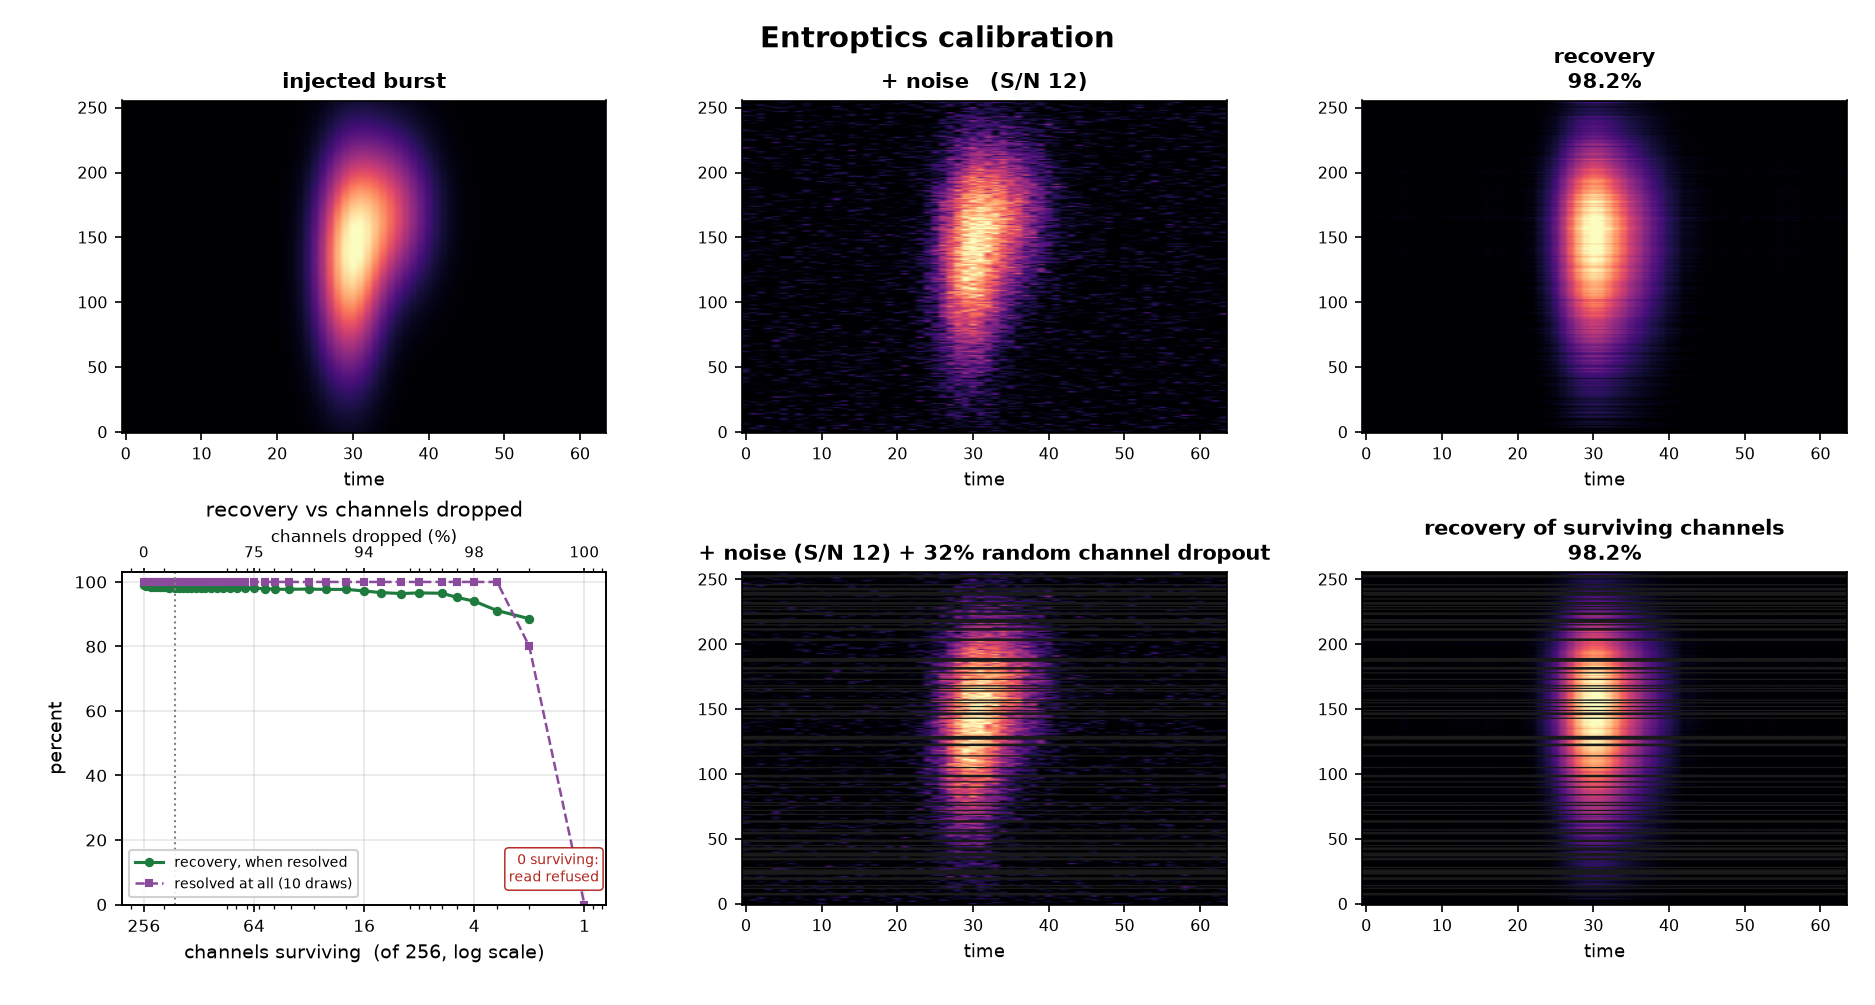
\includegraphics[width=\textwidth,height=0.8\textheight,keepaspectratio]{figures/calibration.png}
\caption*{Figure 1. Read-side filter calibration on a synthetic burst: the
injected burst, the field plus noise, and the recovery (top); recovery
against channel dropout, as two series, swept to one surviving channel
of 256 (bottom).}
\end{figure*}

\emph{A crossing conserves energy and cannot brighten a beam.} Two sides placed on one shared basis through lenses of differing surface width, read in both directions across six étendue ratios. The partition of Proposition A.4 closes to machine precision on all twelve crossings, which is a check on the arithmetic rather than evidence for the proposition: it is an identity in \((E_g,P,\tau)\) and holds for any three numbers. Radiance never rises (12/12), and in every concentrating crossing it is carried across exactly (6/6), which is the equality case of Proposition A.5.

\emph{The lift buys a forecast, and a shuffled control is what shows it.} A logistic map and an amplitude-modulated oscillator, \(T=600\), have no linear one-step map on their own coordinates. In delay coordinates at \(d=24\) the operator forecasts a held-out tail at \(0.074\) and \(0.040\) of persistence, against \(0.492\) and \(0.527\) for the same trajectories in a random order --- a separation of \(6.6\times\) and \(13.4\times\). The resolved dimension does not carry this claim: the shuffled logistic trajectory resolves 15 modes against the real one's 5, because the count rises with the observable's dimension \(d\cdot F\) and with whiteness. Order is what the forecast reads, and disorder is what it refuses.

\emph{Order is detected by the permutation null, not by an entropy rate.} Repeat-probability chains over an alphabet of 4, \(N=4000\): an i.i.d. sequence reads \(|z|=1.7\) against its own permutation ensemble and is not called ordered, while the same read at repeat probability \(0.95\) gives \(|z|=2276\), monotonically through \(141\), \(601\) and \(1238\) at intermediate strengths. The first-order entropy is \(2.00\) bits throughout, so the departure is carried entirely by \(n\ge 2\) --- a permutation preserves symbol frequencies exactly, and only the ordering is destroyed. The saturation of Proposition B.2 is exhibited alongside: \(\mathrm H_n\) turns toward \(\log_2(N-n+1)\) as the word count passes the window count, at \(n=6\) for this alphabet and length.

\emph{Structure is reported at the scale that contains it.} A single ordered mode of known period over a unit noise floor, \(T=512\), \(F=24\), swept over trailing windows. The resolved window of Definition 3.6 does not fall as the planted period rises across \(16,32,64,128\) (resolved windows \(8,8,8,17\); Spearman \(+0.77\), the three shortest periods tied), and every period resolves in a window shorter than itself: a partial period of a carrier shared across \(24\) channels is already a mode at this amplitude. The window a structure needs is set by its strength as well as its extent.

\emph{The reads divide by the measured extent, and a mask is not a zero (Def 2.1).} A rank-3 signal at \((T,F)=(200,256)\) with 0--90\% of its channels blanked, 20 draws per fraction. Taken through NaN or through a mask over a finite wrong value, \(\varphi_F\), \(\varphi_T\), \(\varphi\), \(\mathcal E\) and the Strehl ratio all match the same frame with those channels \emph{deleted} to \(3.3\times10^{-16}\) --- floating-point equality, on frames whose nominal width is up to ten times their measured extent. Substituting \(0\) for the same channels is a different measurement and reads as one: \(\varphi_F\) moves by \(0.006\), \(0.018\), \(0.051\) and \(0.137\) at 25\%, 50\%, 75\% and 90\% blanked, rising with the fraction blanked because that is the factor \(L_a/L_{\mathrm{eff}}\) the extent corrects.

\emph{A read is a property of the signal, not of the units it was recorded in (Def 8.1).} A rank-3 signal at \((T,F)=(300,64)\), multiplied through 42 orders of magnitude of recording scale (\(10^{12}\) to \(10^{-30}\)): \(\varphi\), \(\varphi_T\), \(\varphi_F\), \(\mathcal E\), the Strehl ratio, \(a_\delta\), the focus, \(K_{\mathrm{signal}}\) and the coherence are all invariant to \(5\times10^{-15}\) relative --- \(K_{\mathrm{signal}}=3\) and coherence \(0.343\) at strain scale (\(10^{-21}\)) exactly as at unit scale. Replacing that derived floor with a fixed absolute one --- the value the derived floor itself takes at unit scale, then held constant --- breaks the read at \(7\) of the \(8\) scales: it resolves all \(64\) modes at \(10^{3}\) and above, and none at \(10^{-6}\) and below, against a true \(3\) throughout. It is correct only at the scale it was fixed at. Uniformly quantized over its own range from 16 bits down to 2, the floor moves by at most \(0.2\%\) --- it is drawn from shuffles of the record's own values, and quantization moves it only as far as it moves them --- and the resolved count holds at the planted \(3\) at every depth, down to a four-level staircase at 2 bits.

\emph{Channel scatter separates a decay that is structure from one that is noise (Def 4.8).} An uncorrelated record and an AR(1) record with a planted correlation length \(\rho=8\), \(T=1500\), each read at \(F=4,16,64,256\) channels. On the uncorrelated record the noise and tail shares coincide at every width (ratio \(0.88\)--\(1.05\)): all of the power away from zero lag is channel disagreement. With a correlation length planted they separate by up to \(227\times\) (ratio \(0.237\) falling to \(0.0044\)), so the same tail is read as structure. The scatter falls monotonically with \(F\) in both families (\(0.113\to0.0020\) and \(0.193\to0.0035\)), and the uncorrelated \(a_\delta\) closes on its answer of \(1\) from below as it does (\(0.36\to0.97\)) --- the read is consistent, and the remedy a wide scatter points at is more channels.

\subsection{12.1 Real data: fast radio bursts}\label{121-real-data-fast-radio-bursts}

This section reports what the untuned instrument does on a real substrate. The application is developed at length in a companion preprint {[}Sessford 2026b{]}, which carries the agreement against CHIME's forward model with the two reference points that scale it --- a noise-limited reference and a fold-resolution ceiling --- and states the limits of the comparison in full. What is given here is the evidence that the transfer happens.

The synthetic checks plant a known truth; a real substrate tests whether the \emph{same untuned instrument} transfers. We apply the plain library (zero tuning) to the publicly released CHIME/FRB Catalog-1 waterfalls {[}CHIME/FRB Collaboration 2021; data at the CANFAR archive, CISTI.CANFAR/21.0007{]} at native 16384-channel resolution through the read-side filter (\texttt{figures/\allowbreak{}frb\_\allowbreak{}panel.\allowbreak{}py} in entroptics-frb), which supplies only observer facts: dead channels are dropped --- never zero-filled --- and the surviving channels are passed to the aperture front door. ``Dead'' is the catalogue's own mask together with a zero-variance test, and the surviving width is \(9{,}760\)--\(11{,}696\) of the \(16{,}384\) recorded channels across the four events. The read is then taken at whatever width the guard of Definition 2.2 folds to, which for these frames is \(5{,}949\)--\(10{,}972\) --- the instrument reading at the resolution it judges the record to carry, which is the untuned behaviour and not a choice made for the figure. Each width is recorded per burst in the companion table. The catalog waterfalls arrive already dedispersed; the library adds no dedispersion of its own, and any residual sweep shows as diagonal structure the read catches directly. Everything downstream is the library.

For each burst the filter resolves the signal above the derived noise floor (\(K_{\mathrm{signal}}\ge 1\)) and reconstructs it as the projection onto its resolved modes (Def 8.4): the noise sea stays in the residual, the \(\varphi_F>\varphi_T\) geometry cut moves persistent narrowband interference there too, and the burst morphology is left intact. The modes are read on the folded screen and every recorded channel is projected onto them, so the read is at the recorded frequency resolution. The per-burst reads annotated on each panel --- the resolved count \(K_{\mathrm{signal}}\), the bounded \emph{contrast} \(\sigma_1/\Phi\) (the leading singular value over the screen floor), and the coherence \(z\) of §5 --- report the contrast. The figure routine writes these per-burst values, with the live-channel and RFI counts, to a companion table (\texttt{frb\_\allowbreak{}panel.\allowbreak{}csv}) regenerated from the CANFAR waterfalls. Figure 2 places the entroptics reconstruction beside CHIME's own \emph{fitburst} forward model and the raw waterfall on four bright events, drawn at random from the release and read with no per-substrate tuning. The three are shown side by side for direct comparison, with a fourth panel holding what the read did not keep --- a plain difference from the waterfall, since the read is returned on the waterfall's own amplitude scale. The per-burst reads in \texttt{frb\_\allowbreak{}panel.\allowbreak{}csv} carry the record's shape alongside them --- \(T=19\)--\(38\) against \(16{,}384\) recorded channels --- so the aspect ratio each read was taken at is on the page.

\emph{An independent check on the read.} CHIME's forward model is fitted with the shape of a burst already in it --- Gaussians in time against a running power law in frequency --- and solves for that shape's parameters. The read is given no model of a burst at all, and keeps whatever modes clear the floor. The two share no assumptions, so agreement between them on the same waterfall is evidence that the read is finding the burst rather than an artifact of its own construction.

Correlation against the forward model, every quantity scored on the live channels and with its per-channel baseline removed: the raw waterfall reads \(0.115\)--\(0.373\) (mean \(0.198\)), the read \(0.421\)--\(0.533\) (mean \(0.470\)). The model is smooth along frequency, so a box-average of the raw to the width the modes were read at is scored alongside it --- smoothing alone, with no read. It reads \(0.214\). \textbf{Smoothing accounts for \(6.1\%\) of the gain and the read for the rest.} The read is at the recorded channel resolution, so structure along frequency that the smooth model does not carry is kept in it rather than averaged away. All three columns are in the companion table, per burst.

The baseline removal is what makes the three comparable, and it is applied to all of them. \texttt{model\_\allowbreak{}wfall} carries no per-channel standing level at all --- its per-channel median is numerically zero, at most \(3.9\times10^{-6}\) across the four events against model maxima of \(0.108\)--\(0.506\) --- because it is a statement about the burst and not about each channel's baseline, so a series that carried one would be scored against a series that does not and the baseline would count as disagreement. Centring one series and not the others would hand that one a comparison the references never got.

Neither is ground truth. The source of a fast radio burst is unknown, and the forward model is itself a fit to this same waterfall with no per-channel freedom. The agreement says that two methods assuming nothing in common find the same burst; it does not say either has recovered it correctly.

The panels differ most obviously in how clean they look, and that is the display rather than the data: each is contrast-stretched independently between its own median and 99.7th percentile, and the model is noiseless and non-negative (median \(0\), maximum \(\approx0.5\)) where the waterfall spans \(-0.9\) to \(+7.0\). The comparison to make by eye is therefore of morphology and not of contrast.

One consequence of that stretch looks like an artifact and is not. The raw panel's range is set by its noise, much of which the read leaves in the residual, so the reconstruction's range is narrower --- \(1.0\times\) to \(1.9\times\) across the four events --- and a channel whose standing level sits off its neighbours can saturate against it as a horizontal line. On FRB20190227A three channels clip, and none on the other three events. The worst has a standing level \(3.70\) noise sigma above the frame median: \(1.06\) of the raw panel's range and \(1.43\) of the reconstruction's, so it clips in both. The level is real and the read reproduces it rather than inventing it (raw median \(+0.444\), reconstruction \(+0.555\)); the residual carries \(-0.129\) of it, \(0.86\) standard deviations from that panel's median. The counts and every quantity above are written to \texttt{frb\_\allowbreak{}display.\allowbreak{}csv}, which pins each definition: the span is the panel's own stretch (99.7th percentile less median), the offset is a channel's median in the reconstruction against that panel's frame median, and the noise sigma is \(1.4826\) times the raw frame's median absolute deviation. The read is at the recorded channel resolution, so a level is attributed to the channel that carries it.

A further \textbf{12 waterfalls drawn uniformly at random} from the same public release, at a fixed seed, are read by the identical path (\texttt{figures/\allowbreak{}frb\_\allowbreak{}spotcheck.\allowbreak{}py} in entroptics-frb, table in \texttt{frb\_\allowbreak{}spotcheck.\allowbreak{}csv}). All twelve are read without incident, and \(K_{\mathrm{signal}}\ge1\) on eight of them. The four that resolve nothing are the four whose leading singular value sits at or below the derived floor (contrast \(0.99\)--\(1.00\), against \(1.17\)--\(2.03\) for the events of Figure 2), the floor refusing a mode it cannot separate from the bulk. Record length does not separate the two groups: the four that resolve nothing span \(T=19\)--\(57\) and the eight that resolve span \(T=19\)--\(95\), so the shortest records sit in both. What this establishes is that the untuned instrument runs on records it was not selected against, and reports what it finds on them.

\begin{figure*}[tbp]
\centering
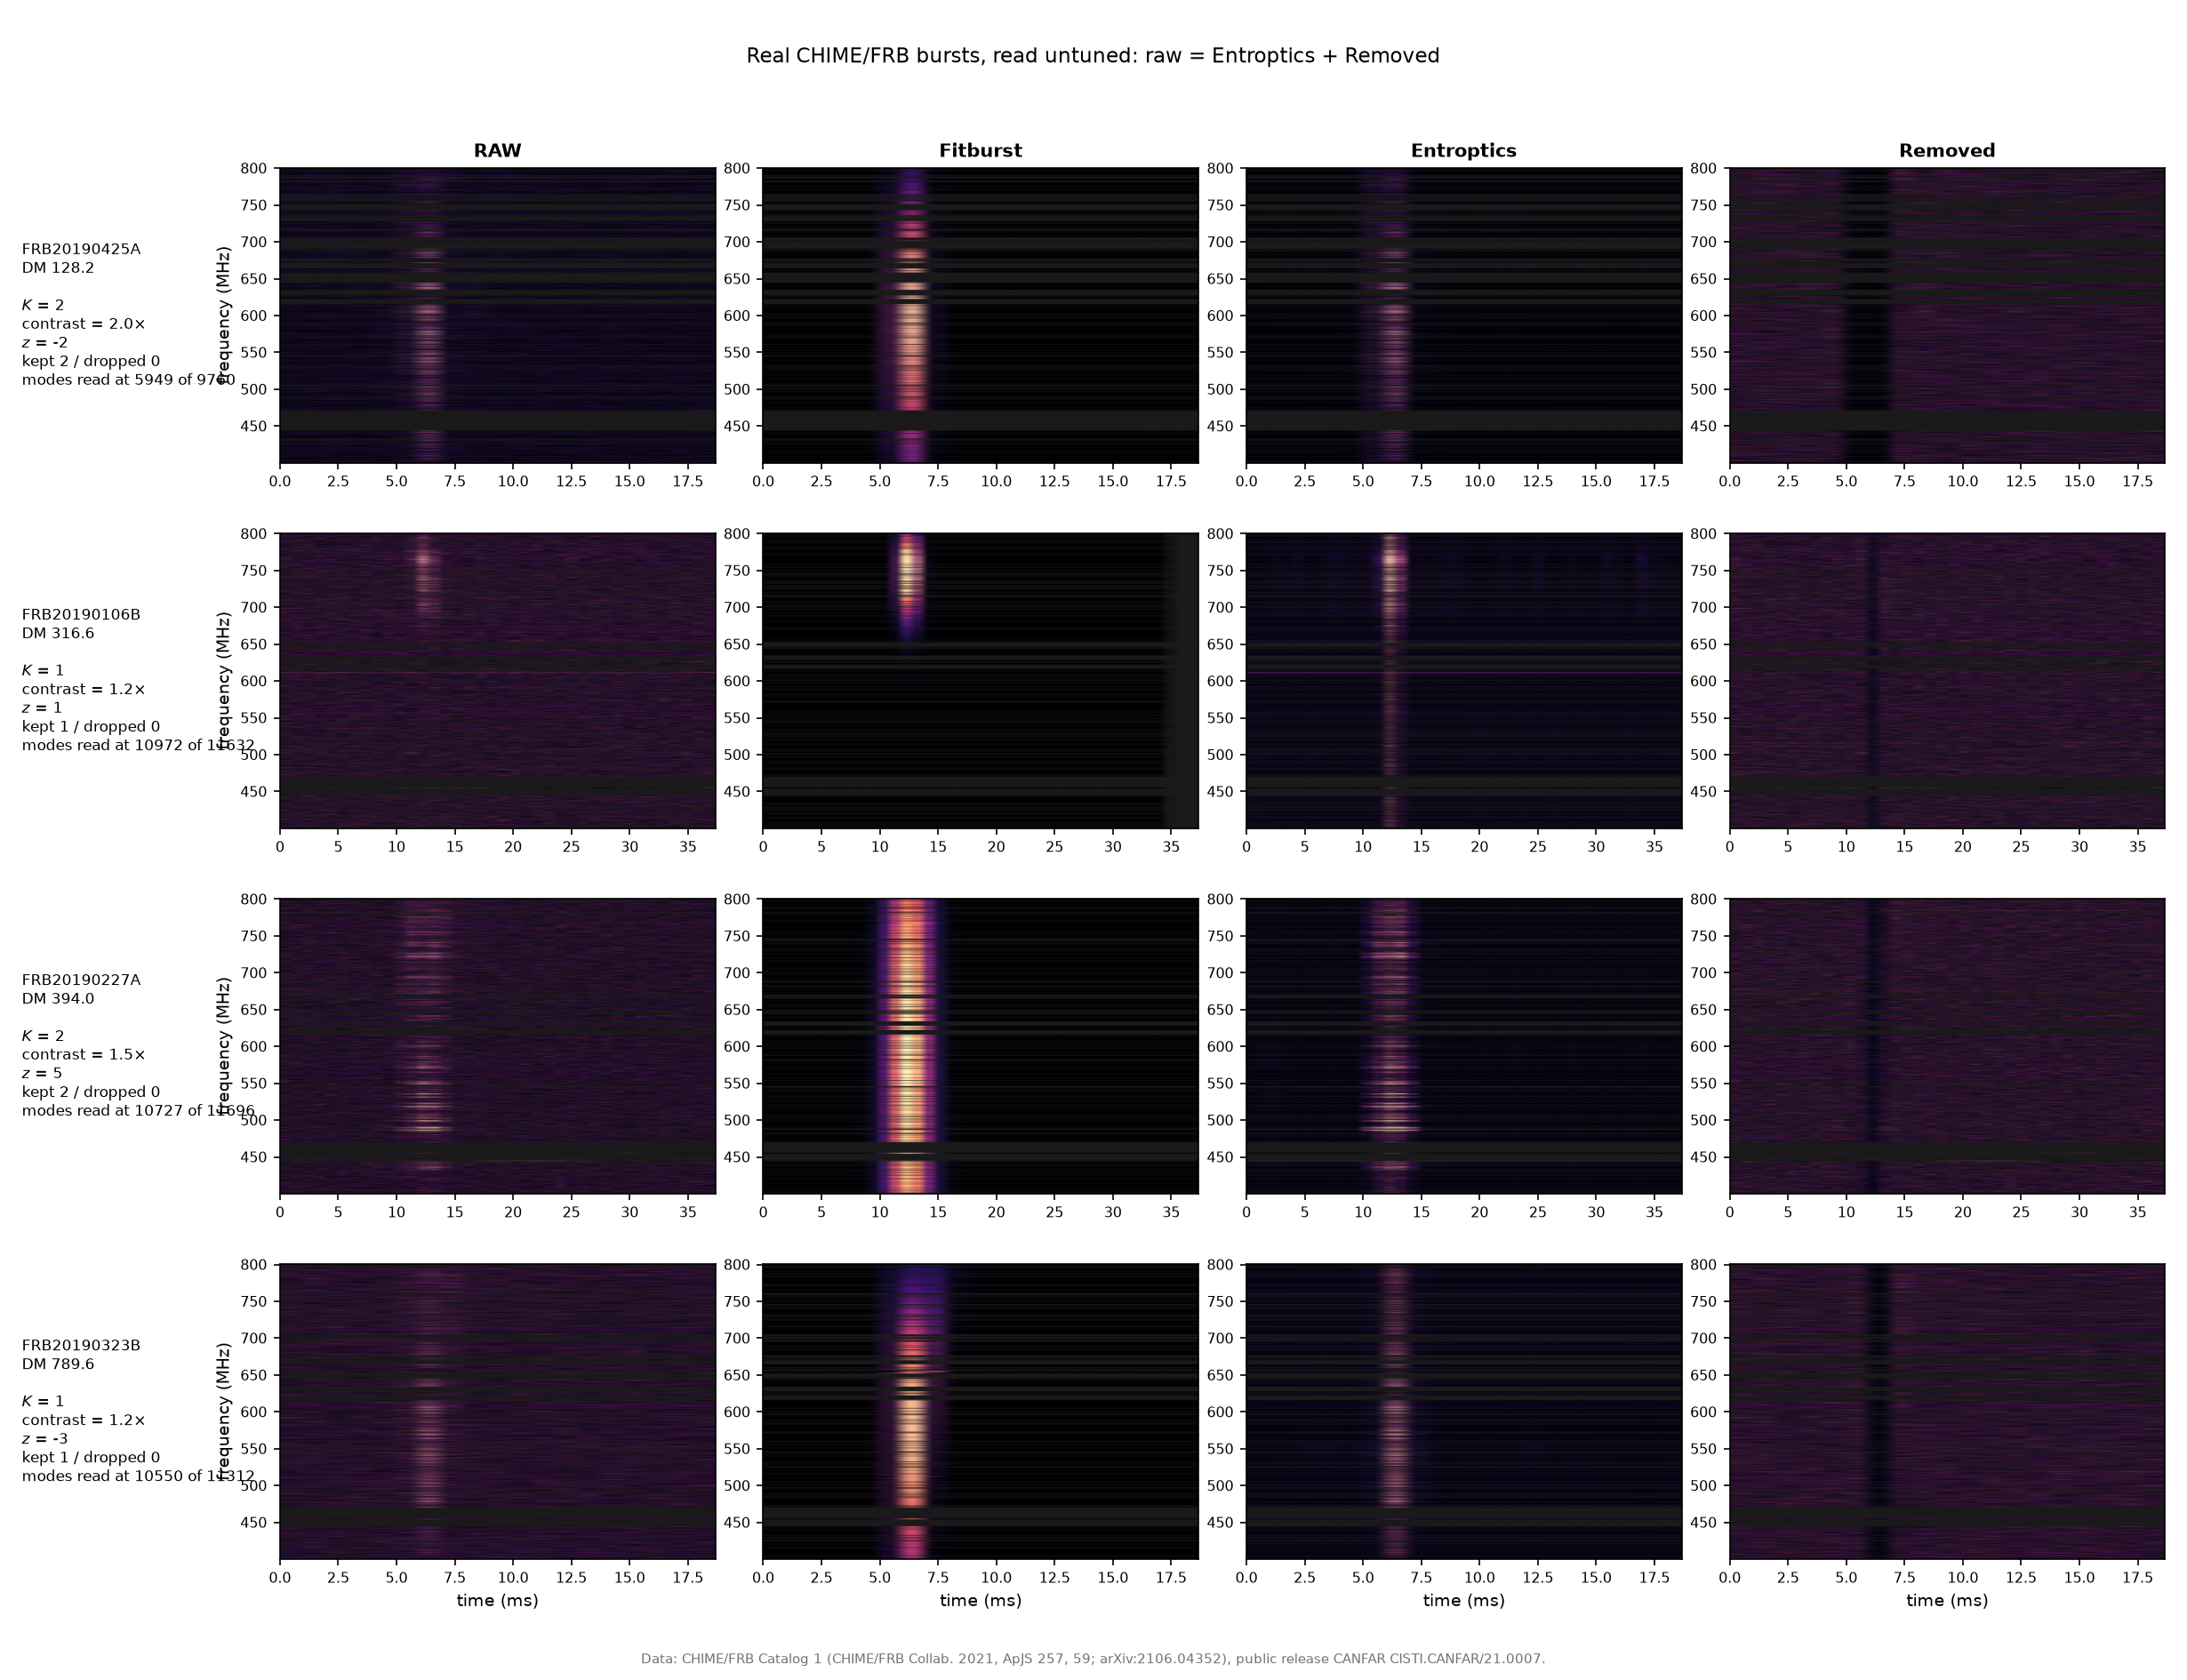
\includegraphics[width=\textwidth,height=0.8\textheight,keepaspectratio]{figures/frb_panel.png}
\caption*{Figure 2. Four CHIME/FRB Catalog-1 bursts read untuned, one row per
event. Left to right: the raw dedispersed waterfall, CHIME's
\emph{fitburst} forward model, the entroptics reconstruction, and what
the read did not keep.}
\end{figure*}

\section{13. Formal verification}\label{13-formal-verification}

Part of the development is machine-checked in Lean 4 / Mathlib: ninety theorems that compile with no \texttt{sorry}, each depending only on the standard axioms \texttt{propext}, \texttt{Classical.\allowbreak{}choice}, and \texttt{Quot.\allowbreak{}sound}. The count is not a measure of coverage --- many are one-line specializations, ring identities, harmonic-sum steps, or aliases of Mathlib results. The development's only definitions are the time-limit, band-limit and concentration operators of the aperture count below and the window they are read on; every other theorem is a claim about explicit sums and matrices, and the identification with the reads above is carried by this paper, not by Lean. What is \textbf{not} certified is as important as what is: Definition 5.3's variance --- the denominator of every \(z\) in the paper --- rests on {[}Cliff \& Ord 1981{]} plus the simulation of §12; so does Definition 2.2's fold guard, the equality cases of Lemmas 3.2 and 3.4, and the strict case of Proposition A.5. Each certified statement is the finite, discrete fact the paper asserts.

\begin{itemize}
\tightlist
\item
  The entropy bound \(\mathrm H(q)\in[0,\log_2 n]\), hence the fill-fraction range \(\varphi=2^{\mathrm H(q)}/n\in[1/n,1]\) (Lemma 3.2), and the Strehl bound \(\mathcal S\in[1/T,1]\) (Lemma 3.4).
\item
  The congruence and orthogonal-conjugation invariance of a fixed correlation operator's spectrum (its characteristic polynomial a similarity invariant), whose data sub-case is the fill fraction's invariance under variable permutation and per-variable phase (Proposition 3.5).
\item
  The positive semidefiniteness of the biased-autocovariance Toeplitz matrix whose entry depends on the lag alone (Lemma 4.2), with the peak-at-zero-lag corollary from its \(2\times2\) minor (Corollary 4.3).
\item
  The discrete scale-invariance of the shape factor through the block-repeat identities \(\mathrm H'=\mathrm H+\log_2 s\) and \(\xi'=s\,\xi\) (Proposition 4.5).
\item
  The crossing partition and the brightness bound, radiance out at most radiance in with equality under concentration (Propositions A.4 and A.5).
\item
  The finite count a finite aperture holds, the discrete form of the concentration results {[}Slepian \& Pollak 1961; Landau \& Pollak 1961{]} behind §3's degrees of freedom: on \(\mathbb Z_N\), with a time-limit \(P_S\) to \(T\) sites and a band-limit \(B_\Omega\) to \(W\) Fourier modes, both orthogonal projections, the concentration operator \(A=P_SB_\Omega P_S\) has \(\operatorname{tr}A=TW/N\) and its spectrum in \([0,1]\). The plunge mass \(\delta=\operatorname{tr}A-\operatorname{tr}A^2\) equals the band-limit's leakage across the aperture's edge; the number of eigenvalues above \(1/2\) is within \(2\delta\) of \(TW/N\); and the Rényi-2 count of the normalized spectrum is at least \(TW/N\) and, when \(2\delta\le TW/N\), at most \(TW/N+2\delta\). For a window of consecutive sites and a band of consecutive modes, \(\delta\le(9+\log\min(T,W))/2\) from the Dirichlet-kernel estimate, so the count is \(TW/N\) to within \(9+\log\min(T,W)\) --- the logarithmic plunge of {[}Landau \& Widom 1980{]}, with its constants computed.
\item
  The permutation-null mean via the two-point stabilizer count \((N-2)!\) (Theorem 5.2).
\item
  The algebra behind the coupling's null moments (Theorem 5.6) --- the four steps below, with the assembly into \(\operatorname{tr}(C_AC_B)/(T-1)\) done on paper above and not in Lean: that summing a function of \(\sigma(i)\) over the symmetric group counts each image exactly \((T-1)!\) times whichever index \(i\) is; the vanishing first moment \(\mathbb E_\pi[S]=0\) for a centred sending side; the same-index second-moment term \(\sum_\sigma A_{\sigma(i)d}A_{\sigma(i)e}=(T-1)!\,(C_A)_{de}\); the independence of the distinct-index term from \emph{which} pair of indices is taken; and its value \(T(T-1)\sum_\sigma f(\sigma 0)g(\sigma 1)=T!\big((\sum f)(\sum g)-\sum_a f_ag_a\big)\). Both moment structures are established by explicit bijections --- the decomposition of a permutation of \(\mathrm{Fin}(n{+}1)\) into its value at \(0\) and a permutation of the rest, and right multiplication by an explicitly constructed carrier permutation. The coefficient identity \(1/T+1/(T(T-1))=1/(T-1)\) and the reduction of the resulting entrywise double sum to \(\operatorname{tr}(C_AC_B)\) for symmetric Gram matrices are certified alongside.
\item
  The Weyl perturbation bound for the top eigenvalue composed into the certified attenuation interval (Lemma 6.2).
\item
  The per-row phase invariance of the second moment together with an antipodal cloud that separates focus from resultant (Proposition 7.2).
\item
  The monotonicity of the derived noise floor in its significance quantile and the antitone dependence of the resolved dimension on the floor (§8).
\item
  The propagator identity \(P_{yx}=A\,P_{xx}\) with operator recovery \(P_{yx}P_{xx}^{-1}=A\) and shared spectrum (Theorem 9.2), and the accumulator additivity behind splicing (Theorem 9.3).
\end{itemize}

Two certified statements are narrower than their headline. Theorem 9.2 is verified for an invertible accumulator (ordinary inverse \(P_{xx}^{-1}\)); the rank-deficient pseudoin\allowbreak{}verse-\allowbreak{}on-\allowbreak{}a-\allowbreak{}subspace form is proved on paper (§9). The noise-floor monotonicity certifies the floor formula in its quantile argument; the Tracy--Widom law it invokes is cited. The classical limit laws (Tracy--Widom, Marchenko--Pastur, Weyl) are cited, not re-proved. The optical identification of §10 --- that these entropic and spectral quantities are the aperture's fill fraction, étendue, Strehl ratio, OTF, and carrier --- is a definitional dictionary, not a theorem; the certified lemmas bound and relate the quantities without asserting the naming.

\section{14. Conclusion}\label{14-conclusion}

Entroptics reads a signal at the resolution the signal itself dictates. From the entropy of the power marginals we obtain a matched scale; from the singular and correlation spectra, the classical optical invariants; from the biased autocorrelation, an OTF whose entropy width is the diffraction limit, with the Mercer ratio as an internal consistency check that doubles as a nonstationarity flag; and from an online linear operator, the decay rates the entropy width approximates. The governing lemmas are proved above, and those §13 names are machine-checked; the whole is deterministic and backend-portable.

What the construction does not do is worth stating as plainly. The derived floor is calibrated against an i.i.d. bulk: noise correlated across channels, or across rows, is counted as signal, and the calibration of §12 speaks to neither. The resolved count over-reads at extreme aspect ratio. The geometry cut of Definition 8.4 discards persistent structure whether or not that structure is interference. The rates of §9 assume a linear one-step map on a stationary record, and the delay depth of the lift is a stated input. The signal supplies the aperture, the resolution, and the width of the fold; whether to fold at all is decided at a level the caller sets.

\begin{center}\rule{0.5\linewidth}{0.5pt}\end{center}

\typesetpart{Further reads carried by the library}{Further reads carried by the library}

The two appendices below document read families the library carries that are not on the linear
path through the core construction. Each is complete on its own terms and neither is used by
Sections 2--9.

\section{Appendix A. The two-way screen: lenses meeting on a shared basis}\label{appendix-a-the-two-way-screen-lenses-meeting-on-a-shared-basis}

Sections 2--9 read one signal. Two signals meet only if they are carried into one set of coordinates, and the reads that follow are about the crossing.

\textbf{Definition A.1 (Lens and screen)} --- A \emph{lens} is a pair of maps \((\iota_g,\iota_g^{-1})\) for a side \(g\), where \(\iota_g\) carries that side's surface \(S_g\in\mathbb{C}^{T_g\times F_g}\) to a frame \(X_g=\iota_g(S_g)\in\mathbb{C}^{T_g\times D}\) on a shared basis of width \(D\), and \(\iota_g^{-1}\) carries a frame back out. A \emph{screen} is a set of lenses whose entries land on one \(D\), together with the frames they have placed. Each side supplies its own energy law, zero and null; the screen supplies none. With \(N\) sides there are \(N\) conversions and no pairwise table, because every pair meets through the basis.

The ordered axis is each side's own. Reads that pair rows --- the coupling of §5, the joint read --- require a common ordering and say so; reads that meet on the basis alone do not.

\textbf{Definition A.2 (Beam and étendue)} --- The \emph{beam} a side carries is its placed frame read as an aperture: energy \(E_g=\lVert X_g\rVert_F^2\), basis the resolved directions of §8, and étendue \(G_g=\varphi_T\varphi_F\) --- the phase-space area of §3, invariant under the congruences of Lemma 3.4. A beam decomposes into modes, each itself a beam of one, so the same three quantities describe a mode, a bundle and a side.

\textbf{Definition A.3 (Crossing)} --- For an ordered pair \((g\to h)\), the \emph{pertinent} energy \(P\) is the part of \(g\)'s beam that \(h\)'s basis resolves. The \emph{transmissible fraction} is the étendue that fits,

\typesetdisplay{\tau=\min\!\left(1,\ \frac{G_h}{G_g}\right),}{}

and the crossing is written

\typesetdisplay{\underbrace{P\tau}_{\text{absorbed}}\ +\ \underbrace{(E_g-P)}_{\text{bystanding}}\ +\ \underbrace{P(1-\tau)}_{\text{reflected}}\ =\ E_g .}{}

\textbf{Proposition A.4 (The partition closes)} --- The three parts of Definition A.3 sum to the beam's energy identically, for every \(E_g\), \(P\) and \(\tau\). This is a statement about the bookkeeping, not a conservation law: the three parts are \emph{defined} as a split of \(E_g\), and the proposition records that the split is exhaustive and leaves nothing unassigned.

\emph{Proof.} Ring identity in \((E_g,P,\tau)\); verified in Lean (\texttt{crossing\_\allowbreak{}partition}). \(\square\)

Energy that meets a side resolving nothing matching it is \emph{bystanding}: real, present, and pertinent to some other pairing. It is not loss, and it remains available to a further screen.

\textbf{Proposition A.5 (The radiance bound)} --- Let radiance be pertinent energy per unit étendue, \(L_g=P/G_g\) and \(L_h=P\tau/G_h\). For \(G_g,G_h>0\) and \(P\ge 0\),

\typesetdisplay{L_h\ \le\ L_g,}{}

with equality whenever \(G_h\le G_g\), and strictly \(L_h<L_g\) when \(G_h>G_g\) and \(P>0\).

\emph{Proof.} If \(G_h\le G_g\) then \(\tau=G_h/G_g\) and \(L_h=P/G_g=L_g\). Otherwise \(\tau=1\) and \(L_h=P/G_h\le P/G_g\), strictly when \(P>0\). Verified in Lean (\texttt{radiance\_\allowbreak{}le}, \texttt{radiance\_\allowbreak{}eq\_\allowbreak{}of\_\allowbreak{}concentrating}); the strict case is not certified. The equality is not a characterisation --- at \(P=0\) both radiances vanish for every pair of étendues. \(\square\)

The bound follows from how \(\tau\) is defined --- \(\tau=\min(1,G_h/G_g)\) caps what crosses at the receiving side's étendue --- so it is a consequence of the accounting rather than a physical law recovered from it. The classical brightness theorem it is named for rests on measure conservation under a Hamiltonian flow {[}Born \& Wolf 1999{]}; nothing here supplies such a flow, and \(G=\varphi_T\varphi_F\) is a product of entropic fill fractions rather than a phase-space volume. The reading is a deliberate analogy: the accounting is arranged so that a crossing cannot report more pertinent energy per unit étendue than it received.

\textbf{Definition A.6 (Condensation)} --- The absorbed energy itemised over the receiving side's resolved directions. For a quadratic energy law the itemisation is an orthogonal decomposition, so the parts sum to \(P\) and each is the energy of its own frame. The étendue bound fixes how much crosses; it leaves open which directions take it.

\textbf{Definition A.7 (Certificates)} --- Three properties of a lens are read, each on the side's own signal. \emph{Linearity} compares converting a frame's modes together against converting them apart, and converting a scaled frame against scaling the conversion; a departure that survives balancing means the modes interact inside the conversion. \emph{Losslessness} measures the round-trip residual \(\iota_g^{-1}(\iota_g(S))-S\) against the derived floor of §8. A residual below the floor is one this record cannot resolve, which is not the same as one that is not there: the read reports the largest residual it could have missed at the observed \(\hat\sigma\) and shape, and a shorter or noisier record admits a larger one. \emph{Realisation} compares what a crossing delivers through the receiving lens against the étendue bound of Definition A.3, separating conversion loss from the phase-space loss \(\tau\) already accounts for.

\textbf{Definition A.8 (Balance)} --- Each side is brought to its own zero before any read. The residual of the screen's accounting is scored against the same null as §8, so closure is a calibrated decision at the reader's level --- a failure to resolve a residual, reported with the bound it was taken at, and not a demonstration that none exists.

The signed coupling of Theorem 5.6 is the crossing's alignment read, and it is defined only on a shared basis: across two bases the sole basis-free statistic is non-negative and has no exact null, so the screen refuses the pairing.

\section{Appendix B. Symbol sequences: the ordered axis without amplitudes}\label{appendix-b-symbol-sequences-the-ordered-axis-without-amplitudes}

Sections 2--9 and Appendix A read an ordered axis of amplitudes. When the ordered object is a string of symbols from a finite alphabet the question changes: not how many modes stand above the floor, but how much of the next symbol the past already fixes.

\textbf{Definition B.1 (Block entropies)} --- For a sequence over an alphabet \(\mathcal X\), let \(\mathrm H_n\) be the Shannon entropy of the distribution of \(n\)-words. Then

\typesetdisplay{h_n=\mathrm H_{n+1}-\mathrm H_n=\mathrm H(X_{n+1}\mid X_1..X_n),\qquad h_n^{\mathrm{av}}=\mathrm H_n/n,}{\begin{gathered}h_n=\mathrm H_{n+1}-\mathrm H_n=\mathrm H(X_{n+1}\mid X_1..X_n),\\ h_n^{\mathrm{av}}=\mathrm H_n/n,\end{gathered}}

the conditional entropy of the next symbol and the per-symbol average. \(\mathrm H_1\) sees only symbol frequencies; \(\mathrm H_n\) carries every correlation shorter than \(n\).

In the infinite-data limit both descend to the entropy rate \(h\) and bound it from above, \(h_n^{\mathrm{av}}\ge h_n\ge h\) {[}Lesne 2014{]}, with \(h<\mathrm H_1\) exactly when correlations are present.

\textbf{Proposition B.2 (Finite-sequence saturation)} --- On a sequence of length \(N\) the ladder of Definition B.1 does not reach \(h\). Once the number of possible \(n\)-words exceeds the number of observed windows, \(\mathrm H_n\) saturates at \(\log_2(N-n+1)\), and \(h_n\) turns over and descends below \(h\).

\emph{Proof.} At most \(N-n+1\) windows are observed, so the empirical \(n\)-word distribution has support at most \(N-n+1\) and \(\mathrm H_n\le\log_2(N-n+1)\). Beyond that point increments of \(\mathrm H_n\) are bounded by the growth of \(\log_2(N-n+1)\), which tends to zero. \(\square\)

The consequence is stated outright: no single number \(h\) is reported from the ladder. The estimate that a single finite sequence does support is the Lempel--Ziv rate, which converges to \(h\) for a stationary ergodic source {[}Ziv \& Lempel 1978{]}.

\textbf{Definition B.3 (Order surrogate)} --- Compare the block entropies of the sequence against an ensemble drawn by permuting it. A permutation preserves the symbol frequencies exactly and destroys every correlation, so \(\mathrm H_1\) is invariant and \(\mathrm H_n\) for \(n\ge 2\) is not. The standardised departure of \(\mathrm H_n\) from that ensemble is the evidence that order carries information, at the reader's level of §11.1 and with no entropy rate estimated anywhere in the comparison.

This is the coherence of §5 in its symbolic form: the same permutation null, standing in the same relation to the same question --- is the ordering doing work --- read on a distribution over words instead of on a correlation over lags.

\section{Declaration of generative AI use}\label{declaration-of-generative-ai-use}

The author used Anthropic's Claude Opus (versions 4.8, 5, and 5.5) in the preparation of this work. Its
contribution was to write code, and to generate and validate content. The ideas, the construction
and the claims are the author's. No other generative AI tool was used. The author reviewed and
edited all output and takes full responsibility for the content of this publication.

\section{References}\label{references}

\begin{itemize}
\tightlist
\item
  E. Abbe, \emph{Beiträge zur Theorie des Mikroskops und der mikroskopischen Wahrnehmung}, Arch. mikroskop. Anat. \textbf{9} (1873) 413--468.
\item
  Z. Bao, G. Pan, W. Zhou, \emph{Tracy--Widom law for the extreme eigenvalues of sample correlation matrices}, Electron. J. Probab. \textbf{17} (2012) no. 88, 1--32.
\item
  R. G. Baraniuk, P. Flandrin, A. J. E. M. Janssen, O. J. J. Michel, \emph{Measuring time-frequency information content using the Rényi entropies}, IEEE Trans. Inform. Theory \textbf{47} (2001) 1391--1409.
\item
  M. Born, E. Wolf, \emph{Principles of Optics}, 7th ed., Cambridge University Press, 1999.
\item
  F. Bornemann, \emph{On the numerical evaluation of distributions in random matrix theory: a review}, Markov Process. Related Fields \textbf{16} (2010) 803--866.
\item
  L. L. Campbell, \emph{Minimum coefficient rate for stationary random processes}, Information and Control \textbf{3} (1960) 360--371.
\item
  L. L. Campbell, \emph{Exponential entropy as a measure of extent of a distribution}, Z. Wahrsche\allowbreak{}inlichke\allowbreak{}itstheor\allowbreak{}ie verw. Gebiete \textbf{5} (1966) 217--225.
\item
  CHIME/FRB Collaboration, \emph{The First CHIME/FRB Fast Radio Burst Catalog}, Astrophys. J. Suppl. Ser. \textbf{257} (2021) 59, arXiv:2106.04352. Data (public): CANFAR archive, CISTI.CANFAR/21.0007, \url{https://www.canfar.net/}.
\item
  A. D. Cliff, J. K. Ord, \emph{Spatial Processes: Models and Applications}, Pion, 1981.
\item
  K. R. Davidson, S. J. Szarek, \emph{Local operator theory, random matrices and Banach spaces}, in: Handbook of the Geometry of Banach Spaces, Vol. I, North-Holland, 2001, pp. 317--366.
\item
  L. De Lathauwer, B. De Moor, J. Vandewalle, \emph{A multilinear singular value decomposition}, SIAM J. Matrix Anal. Appl. \textbf{21} (2000) 1253--1278.
\item
  M. Dwass, \emph{Modified randomization tests for nonparametric hypotheses}, Ann. Math. Statist. \textbf{28} (1957) 181--187.
\item
  P. L. Ferrari and H. Spohn, \emph{A determinantal formula for the GOE Tracy--Widom distribution}, J. Phys. A \textbf{38} (2005) L557--L561.
\item
  D. Gabor, \emph{Theory of communication}, J. IEE \textbf{93} (1946) 429--457.
\item
  M. Gavish, D. L. Donoho, \emph{The optimal hard threshold for singular values is \(4/\sqrt{3}\)}, IEEE Trans. Inform. Theory \textbf{60} (2014) 5040--5053.
\item
  J. W. Goodman, \emph{Introduction to Fourier Optics}, 3rd ed., Roberts \& Co., 2005.
\item
  N. Halko, P. G. Martinsson, J. A. Tropp, \emph{Finding structure with randomness: probabilistic algorithms for constructing approximate matrix decompositions}, SIAM Rev. \textbf{53} (2011) 217--288.
\item
  N. J. Higham, \emph{Accuracy and Stability of Numerical Algorithms}, 2nd ed., SIAM, 2002.
\item
  W. Hoeffding, \emph{A combinatorial central limit theorem}, Ann. Math. Statist. \textbf{22} (1951) 558-566.
\item
  A. C. A. Hope, \emph{A simplified Monte Carlo significance test procedure}, J. R. Statist. Soc. B \textbf{30} (1968) 582--598.
\item
  T. Jiang, \emph{The limiting distributions of eigenvalues of sample correlation matrices}, Sankhyā A \textbf{66} (2004) 35--48.
\item
  I. M. Johnstone, \emph{On the distribution of the largest eigenvalue in principal components analysis}, Ann. Statist. \textbf{29} (2001) 295--327.
\item
  J. Josse, J. Pagès, F. Husson, \emph{Testing the significance of the RV coefficient}, Comput. Statist. Data Anal. \textbf{53} (2008) 82--91.
\item
  F. Kazi-Aoual, S. Hitier, R. Sabatier, J.-D. Lebreton, \emph{Refined approximations to permutation tests for multivariate inference}, Comput. Statist. Data Anal. \textbf{20} (1995) 643--656.
\item
  M. H. Kassner, \emph{Screens for the absorption of micro-wave radiation}, M.Sc. thesis, Dept. of Physics, McGill University, 1950. \href{https://doi.org/10.82308/34546}{https:\allowbreak{}/\allowbreak{}/\allowbreak{}doi.\allowbreak{}org/\allowbreak{}10.\allowbreak{}82308/\allowbreak{}34546}
\item
  A. Khinchin, \emph{Korrelationstheorie der stationären stochastischen Prozesse}, Math. Ann. \textbf{109} (1934) 604--615.
\item
  B. O. Koopman, \emph{Hamiltonian systems and transformation in Hilbert space}, Proc. Natl. Acad. Sci. USA \textbf{17} (1931) 315--318.
\item
  S. Kornblith, M. Norouzi, H. Lee, G. Hinton, \emph{Similarity of neural network representations revisited}, Proc. 36th Int. Conf. Machine Learning (ICML), PMLR \textbf{97} (2019), arXiv:1905.00414.
\item
  H. J. Landau, H. O. Pollak, \emph{Prolate spheroidal wave functions, Fourier analysis and uncertainty II}, Bell Syst. Tech. J. \textbf{40} (1961) 65--84.
\item
  H. J. Landau, H. Widom, \emph{Eigenvalue distribution of time and frequency limiting}, J. Math. Anal. Appl. \textbf{77} (1980) 469--481.
\item
  A. Lesne, \emph{Shannon entropy: a rigorous notion at the crossroads between probability, information theory, dynamical systems and statistical physics}, Math. Struct. Comp. Sci. \textbf{24} (2014) e240311.
\item
  W. Lukosz, \emph{Optical systems with resolving powers exceeding the classical limit}, J. Opt. Soc. Am. \textbf{56} (1966) 1463--1472.
\item
  V. A. Marchenko, L. A. Pastur, \emph{Distribution of eigenvalues for some sets of random matrices}, Math. USSR-Sb. \textbf{1} (1967) 457--483.
\item
  K. V. Mardia, P. E. Jupp, \emph{Directional Statistics}, Wiley, 2000.
\item
  J. Mercer, \emph{Functions of positive and negative type, and their connection with the theory of integral equations}, Phil. Trans. R. Soc. Lond. A \textbf{209} (1909) 415--446.
\item
  N. S. Pillai, J. Yin, \emph{Edge universality of correlation matrices}, Ann. Statist. \textbf{40} (2012) 1737--1763.
\item
  P. Robert, Y. Escoufier, \emph{A unifying tool for linear multivariate statistical methods: the RV-coefficient}, J. R. Statist. Soc. C (Applied Statistics) \textbf{25} (1976) 257--265.
\item
  O. Roy, M. Vetterli, \emph{The effective rank: a measure of effective dimensionality}, Proc. 15th European Signal Processing Conf. (EUSIPCO) (2007) 606--610.
\item
  I. J. Sessford, \emph{Exact permutation-null moments for a signed bilinear coupling statistic on a shared basis}, pre-print, 2026a. \texttt{research/\allowbreak{}supplemental/\allowbreak{}coupling/\allowbreak{}PAPER\_\allowbreak{}coupling.\allowbreak{}md}.
\item
  I. J. Sessford, \emph{An untuned rank-selection and reconstruction procedure recovers CHIME/FRB burst morphology}, pre-print, 2026b. \href{https://github.com/Agience/entroptics-frb}{https:\allowbreak{}/\allowbreak{}/\allowbreak{}github.\allowbreak{}com/\allowbreak{}Agience/\allowbreak{}entropti\allowbreak{}cs-\allowbreak{}frb}
\item
  C. E. Shannon, \emph{A Mathematical Theory of Communication}, Bell Syst. Tech. J. \textbf{27} (1948) 379--423, 623--656.
\item
  D. Slepian, H. O. Pollak, \emph{Prolate spheroidal wave functions, Fourier analysis and uncertainty I}, Bell Syst. Tech. J. \textbf{40} (1961) 43--63.
\item
  F. Takens, \emph{Detecting strange attractors in turbulence}, in: Dynamical Systems and Turbulence, Lecture Notes in Mathematics \textbf{898}, Springer, 1981, pp. 366--381.
\item
  G. Toraldo di Francia, \emph{Degrees of freedom of an image}, J. Opt. Soc. Am. \textbf{59} (1969) 799--804.
\item
  C. A. Tracy, H. Widom, \emph{Level-spacing distributions and the Airy kernel}, Comm. Math. Phys. \textbf{159} (1994) 151--174.
\item
  C. A. Tracy, H. Widom, \emph{On orthogonal and symplectic matrix ensembles}, Comm. Math. Phys. \textbf{177} (1996) 727--754.
\item
  J. H. Tu, C. W. Rowley, D. M. Luchtenburg, S. L. Brunton, J. N. Kutz, \emph{On dynamic mode decomposition: theory and applications}, J. Comput. Dyn. \textbf{1} (2014) 391--421.
\item
  L. R. Tucker, \emph{Some mathematical notes on three-mode factor analysis}, Psychometrika \textbf{31} (1966) 279--311.
\item
  J. W. Tukey, \emph{Exploratory Data Analysis}, Addison-Wesley, 1977.
\item
  H. Weyl, \emph{Das asymptotische Verteilungsgesetz der Eigenwerte linearer partieller Differentialgleichungen}, Math. Ann. \textbf{71} (1912) 441--479.
\item
  E. T. Whittaker, \emph{On the functions which are represented by the expansions of the interpolation-theory}, Proc. R. Soc. Edinburgh \textbf{35} (1915) 181--194.
\item
  N. Wiener, \emph{Generalized harmonic analysis}, Acta Math. \textbf{55} (1930) 117--258.
\item
  E. B. Wilson, M. M. Hilferty, \emph{The distribution of chi-square}, Proc. Natl. Acad. Sci. USA \textbf{17} (1931) 684--688.
\item
  E. Wolf, \emph{New theory of partial coherence in the space--frequency domain. Part I: spectra and cross spectra of steady-state sources}, J. Opt. Soc. Am. \textbf{72} (1982) 343--351.
\item
  J. Ziv, A. Lempel, \emph{Compression of individual sequences via variable-rate coding}, IEEE Trans. Inform. Theory \textbf{24} (1978) 530--536.
\end{itemize}

\end{document}
